\documentclass[10pt,letterpaper]{article}
\usepackage[T1]{fontenc}
\usepackage[margin=0.8in]{geometry}
\usepackage{lmodern}
\usepackage{array,booktabs,longtable}
\usepackage{graphicx}
\usepackage{caption}
\usepackage[section]{placeins}
\usepackage{xurl}
\usepackage[hidelinks]{hyperref}
\setlength{\parindent}{0pt}
\setlength{\parskip}{0.5em}
\setlength{\LTpre}{0.5em}
\setlength{\LTpost}{0.8em}
\setlength{\emergencystretch}{2em}
\captionsetup{font=small,labelfont=bf,skip=5pt,hypcap=false}
\title{Mathematical Reasoning with Verifiable Rewards\\Experimental Results Atlas}
\author{Tuan Minh Pham, Tri Vo, Yahor Lechanka\\Purdue University}
\date{Evidence Snapshot: November 23, 2026}
\begin{document}
\maketitle
\begin{center}
Training dynamics, optimization and reward ablations, inference behavior, and benchmarks.
\end{center}
\section{Experimental Setup: Model and Architecture}

This document reports the completed Qwen2.5-Math-1.5B study, not the earlier 7B agent prototype. All primary RL comparisons start from the same pretrained base checkpoint, not Qwen-Math-Instruct and not a previously supervised adapter. The unchanged base checkpoint is the no-RL control. The core question is how outcome-reward training, optimization choices and inference-time sampling change mathematical reasoning.

\begingroup\footnotesize\setlength{\tabcolsep}{3pt}
\begin{longtable}{>{\raggedright\arraybackslash}p{0.2610\linewidth}>{\raggedright\arraybackslash}p{0.6390\linewidth}}
\caption{Model architecture and parameter-update design, verified against the saved model configuration and RL run.}\\
\toprule Component & Specification \\
\midrule\endfirsthead
\toprule Component & Specification \\
\midrule\endhead
\midrule\multicolumn{2}{r}{Continued on next page}\endfoot
\bottomrule\endlastfoot
Backbone & Qwen2.5-Math-1.5B; approximately 1.5 billion parameters; decoder-only causal Transformer \\
Transformer depth /\allowbreak{} hidden width & 28 layers /\allowbreak{} 1536 hidden units \\
Attention & 12 query heads; 2 key/\allowbreak{}value heads (grouped-query attention) \\
Feed-forward width & 8960 \\
Vocabulary /\allowbreak{} context window & 151,936 tokens /\allowbreak{} 4,096 positions \\
RL trainable parameters & Full model; no LoRA adapter and no quantization in the primary RL study \\
Numerical precision & FP32 trainable/\allowbreak{}master weights; BF16 forward/\allowbreak{}backward compute; gradient checkpointing \\
Auxiliary models & No trained critic, learned reward model or prompt-based verifier in the RL objective; frozen reference policy only in nonzero-KL arms \\
\end{longtable}\endgroup


\begin{center}\fbox{\begin{minipage}{.91\linewidth}\centering MATH problem $\rightarrow$ Qwen policy $\rightarrow$ $G$ sampled solutions\\Extract final answers $\rightarrow$ rule-based correctness rewards\\Within-problem relative advantages $\rightarrow$ clipped policy update\end{minipage}}\end{center}

The policy generates complete reasoning responses, and the reward evaluates only the extracted final answer. Training updates the model parameters; it is not few-shot prompting. The main evaluation pipeline does not insert retrieved solutions, run a verifier/revision loop or perform proof-tree search. Inference ablations reuse trained checkpoints and vary decoding or answer selection without further parameter updates.

The tokenizer's chat template renders a system message and the problem as a user message. The fixed system instruction is: \texttt{Please reason step by step, and put your final answer within \textbackslash boxed\{\}.} The same core prompt is used for RL and its ordinary evaluation; wording variants are isolated inference ablations.

The saved primary runtime records TRL 0.25.1, Transformers 4.57.1, PyTorch 2.7.1+cu118 and Math-Verify 0.8.0. These identify the implemented backend, not a claim to reproduce every component of an external paper's training recipe.

\clearpage

\section{Datasets, Development Split and Separation}

The original MATH benchmark contains 7,500 training and 5,000 test problems in our saved snapshot. We filter the original training split to Levels 3--5, require parseable reference answers and prompts no longer than 1,024 tokens, and deduplicate whitespace-normalized problem text. This leaves 5,579 eligible problems. A category/difficulty-balanced development set is reserved first with split seed 42; the RL training subset is selected only from the remaining problems.

\begingroup\footnotesize\setlength{\tabcolsep}{3pt}
\begin{longtable}{>{\raggedright\arraybackslash}p{0.1620\linewidth}>{\raggedright\arraybackslash}p{0.2880\linewidth}>{\raggedright\arraybackslash}p{0.1350\linewidth}>{\raggedright\arraybackslash}p{0.3150\linewidth}}
\caption{Data actually used: development is a custom MATH-train holdout, not MATH-500.}\\
\toprule Dataset /\allowbreak{} partition & Source & Size & Use \\
\midrule\endfirsthead
\toprule Dataset /\allowbreak{} partition & Source & Size & Use \\
\midrule\endhead
\midrule\multicolumn{4}{r}{Continued on next page}\endfoot
\bottomrule\endlastfoot
RL training & Original MATH train, eligible Levels 3--5 & 512 problems & Parameter updates; same fixed problem pool across primary RL arms \\
Dev300 & Reserved original MATH train, Levels 3--5 & 300 problems & Hyperparameter comparisons and checkpoint monitoring; no training updates \\
Dev100 & Fixed subset of Dev300 & 100 problems & Sampled exploration, inference-budget, prompt and selection diagnostics \\
MATH-500 & HuggingFaceH4/\allowbreak{}MATH-500; selected from original MATH test & 500 problems & External competition-math evaluation \\
GSM8K-100 & Fixed 100-problem subset of GSM8K test & 100 problems & External arithmetic/\allowbreak{}word-problem evaluation \\
AIME 2025 & math-ai/\allowbreak{}aime25 test; AIME I + II & 30 problems & External hard competition-math evaluation \\
AIME 2026 & math-ai/\allowbreak{}aime26 test; AIME I + II & 30 problems & External hard competition-math evaluation \\
Retention probes & WikiText subset; BoolQ; ARC-Easy & 32 text blocks; 100 questions per task & Perplexity and raw/\allowbreak{}chat label-likelihood checks, not full-benchmark claims \\
\end{longtable}\endgroup


\textbf{Where dev comes from.} Dev300 and Training512 are two disjoint subsets of the original MATH \emph{training} split. MATH-500 comes from the original MATH \emph{test} split. Dev100 is contained within Dev300, so those two diagnostic cohorts are intentionally not independent. The 512-problem pool is the completed pilot/stabilization study; the larger training-data target in the research plan is not presented as completed training here.

\begingroup\footnotesize\setlength{\tabcolsep}{3pt}
\begin{longtable}{>{\raggedright\arraybackslash}p{0.6750\linewidth}>{\raggedright\arraybackslash}p{0.2250\linewidth}}
\caption{Direct overlap audit of the saved cohorts, using whitespace-normalized problem-text hashes.}\\
\toprule Comparison & Shared problems \\
\midrule\endfirsthead
\toprule Comparison & Shared problems \\
\midrule\endhead
\midrule\multicolumn{2}{r}{Continued on next page}\endfoot
\bottomrule\endlastfoot
Training512 versus Dev300 & 0 \\
Training512 versus MATH-500 & 0 \\
Dev300 versus MATH-500 & 0 \\
\end{longtable}\endgroup


This audit establishes no exact normalized-text overlap among those saved cohorts; it does not rule out semantic near-duplicates or exposure in the base model's pretraining. Development results guide tuning, and external benchmark results have also been inspected across experiments: external does not mean untouched confirmatory data. Each AIME year contains 15 AIME I and 15 AIME II problems; pooled AIME uses 60 distinct problems, so small accuracy changes correspond to few questions.

\clearpage

\section{Algorithms and Training Parameters}

\begingroup\footnotesize\setlength{\tabcolsep}{3pt}
\begin{longtable}{>{\raggedright\arraybackslash}p{0.1620\linewidth}>{\raggedright\arraybackslash}p{0.7380\linewidth}}
\caption{Implemented objectives and controls used in the completed comparison.}\\
\toprule Method & Training signal and update \\
\midrule\endfirsthead
\toprule Method & Training signal and update \\
\midrule\endhead
\midrule\multicolumn{2}{r}{Continued on next page}\endfoot
\bottomrule\endlastfoot
No RL & Untouched Qwen2.5-Math-1.5B base; identical ordinary evaluation prompt and decoding \\
GRPO & Within-problem mean-centered, group-standardized rewards; token-level importance ratios and response-length-normalized clipped policy loss \\
Dr. GRPO & Mean-centered rewards without group-standard-deviation scaling; token-level ratios and fixed maximum-completion-length loss normalization \\
DAPO-style & Group-standardized rewards; token-level ratios; batch-token loss normalization; asymmetric clipping distances 0.2 /\allowbreak{} 0.28 \\
GSPO & Group-standardized rewards; sequence-level importance ratios; clipping distances 0.0003 /\allowbreak{} 0.0004 \\
SFT & Assistant-only cross entropy on human reference solutions; a supervised control, not reinforcement learning \\
RFT & Assistant-only cross entropy on correctness-verified base-model samples; rejection-sampling fine-tuning, not a new RL objective \\
\end{longtable}\endgroup


For a group of $G$ sampled solutions, GRPO uses relative advantages proportional to $(r_i-\bar r)/(s_r+\epsilon)$; Dr.~GRPO uses $r_i-\bar r$ without reward-standard-deviation scaling. DAPO-style and GSPO are the implemented objective variants above, not full-paper reproductions. In particular, the DAPO-style arm does not add dynamic sampling. Loss and gradient-norm scales differ across objectives and should not be ranked directly. PPO and REINFORCE are not completed arms of this study.

\begingroup\footnotesize\setlength{\tabcolsep}{3pt}
\begin{longtable}{>{\raggedright\arraybackslash}p{0.2430\linewidth}>{\raggedright\arraybackslash}p{0.6570\linewidth}}
\caption{Shared RL defaults and the tuned continuation setting.}\\
\toprule Parameter & Value /\allowbreak{} interpretation \\
\midrule\endfirsthead
\toprule Parameter & Value /\allowbreak{} interpretation \\
\midrule\endhead
\midrule\multicolumn{2}{r}{Continued on next page}\endfoot
\bottomrule\endlastfoot
Initialization and data & Same base checkpoint and frozen 512-problem MATH pool; no-RL control has no updates \\
Learning rate /\allowbreak{} schedule & Original method comparison: 1e-6; tuned GRPO continuation: 3e-6; constant schedule, zero warmup \\
Optimizer & AdamW; betas 0.9 /\allowbreak{} 0.95; weight decay 0; gradient-norm clipping at 1.0 \\
Prompt /\allowbreak{} response caps & 1,024 /\allowbreak{} 3,000 tokens \\
Training generation & G=4 independent responses per problem; temperature 1.0; top-p 1.0; top-k disabled \\
Rollout batch & 16 distinct prompts x 4 responses = 64 generated responses \\
Optimizer batch & Microbatch 1; accumulation 16; 16 responses per update \\
Update budget & 128 updates per pass over the 512 problems at G=4; continuation checkpoints at 256 and 512 total updates \\
Clipping /\allowbreak{} KL & GRPO/\allowbreak{}Dr. GRPO: 0.2 /\allowbreak{} 0.2; DAPO-style: 0.2 /\allowbreak{} 0.28; GSPO: 0.0003 /\allowbreak{} 0.0004; KL beta 0 unless ablated; one iteration per generation batch \\
Reference run & Training seed 0; split seed 42; reference-run presentation, not cross-seed averages \\
\end{longtable}\endgroup


The default 64-response rollout batch supplies four 16-response optimizer updates; it is not a batch of 64 distinct problems. Extending to 512 updates revisits the same training pool for four passes rather than introducing 2,048 distinct training problems. Group-size ablations retain the same 512 problems but change generated responses and updates, so they are not compute-matched.

\clearpage

\section{Ablation Design and Evaluation Protocol}

\begingroup\footnotesize\setlength{\tabcolsep}{3pt}
\begin{longtable}{>{\raggedright\arraybackslash}p{0.2070\linewidth}>{\raggedright\arraybackslash}p{0.6930\linewidth}}
\caption{Actual ablation axes; parameters not named in an arm remain at its stated reference setting.}\\
\toprule Study & Values /\allowbreak{} controlled change \\
\midrule\endfirsthead
\toprule Study & Values /\allowbreak{} controlled change \\
\midrule\endhead
\midrule\multicolumn{2}{r}{Continued on next page}\endfoot
\bottomrule\endlastfoot
Learning rate & All four algorithms: 2e-7, 5e-7, 1e-6; GRPO and Dr. GRPO additionally 2e-6, 3e-6; 128-update comparison \\
KL /\allowbreak{} clipping & GRPO at LR 1e-6: KL beta 0, 0.001 or 0.01; symmetric clip distance 0.1, 0.2 or 0.3; one factor changed at a time \\
Reward design & GRPO at LR 3e-6: correctness only; correctness + format bonus; correctness - length penalty \\
Training exploration & At LR 3e-6: temperature 0.7, 1.0 or 1.3 with G=4; G=2, 4 or 8 with temperature 1.0 \\
Training duration & Tuned GRPO at 128, 256 and 512 total updates; same 512-problem pool \\
Inference only & Greedy caps 512 /\allowbreak{} 1,024 /\allowbreak{} 2,048 /\allowbreak{} 3,000; eight-candidate temperatures 0.4 /\allowbreak{} 0.7 /\allowbreak{} 1.0; saved-candidate budgets 1 /\allowbreak{} 2 /\allowbreak{} 4 /\allowbreak{} 8; isolated prompt-wording and selection-rule changes \\
\end{longtable}\endgroup


Let $C$ be binary final-answer correctness, $F$ indicate exactly one nonempty parseable boxed answer, and $L$ be completion length. The rewards are $R_0=C$, $R_{\rm format}=C+0.10F$, and $R_{\rm length}=C-0.05\min(L/3000,1)$. Correctness uses the existing final-answer extractor, whitespace-normalized equality and Math-Verify equivalence fallback; extraction/verification failures receive zero. It is not a learned verifier score or a proof-validity reward. Raw correctness and shaping components are logged separately.

\begingroup\footnotesize\setlength{\tabcolsep}{3pt}
\begin{longtable}{>{\raggedright\arraybackslash}p{0.2160\linewidth}>{\raggedright\arraybackslash}p{0.1440\linewidth}>{\raggedright\arraybackslash}p{0.1080\linewidth}>{\raggedright\arraybackslash}p{0.0810\linewidth}>{\raggedright\arraybackslash}p{0.0990\linewidth}>{\raggedright\arraybackslash}p{0.2520\linewidth}}
\caption{Supervised follow-up configuration: target responses are not necessarily distinct source problems.}\\
\toprule Control & Training targets & LR & Epochs & Opt. batch & Adaptation \\
\midrule\endfirsthead
\toprule Control & Training targets & LR & Epochs & Opt. batch & Adaptation \\
\midrule\endhead
\midrule\multicolumn{6}{r}{Continued on next page}\endfoot
\bottomrule\endlastfoot
Original full SFT & 512 & 1e-05 & 1 & 4 & Full parameters \\
Full SFT & 512 & 5e-06 & 3 & 16 & Full parameters \\
Full RFT & 967 & 5e-06 & 3 & 16 & Full parameters \\
LoRA SFT & 512 & 0.0001 & 3 & 16 & LoRA r=64, alpha=128 \\
Full RFT, filtered & 655 & 5e-06 & 3 & 16 & Full parameters \\
LoRA RFT, filtered & 655 & 0.0001 & 3 & 16 & LoRA r=64, alpha=128 \\
\end{longtable}\endgroup


The supervised follow-ups use a cosine schedule, 3\% warmup, microbatch 1 with accumulation 16, a 4,096-token total sequence cap and assistant-only labels ending at the chat-end token. The original historical full-SFT control instead uses one epoch, LR 1e-5 and optimizer batch 4; it is not pooled with the three-epoch follow-up. LoRA targets attention and MLP projection layers and is merged for evaluation. RFT target counts can exceed 512 because a source problem can contribute multiple verified responses; filtering reduces 967 to 655 targets. Only independently complete evaluation cohorts are scored.

Ordinary benchmark decoding is greedy (temperature 0), cap 3,000, with common end-of-text/chat-end stopping. Sampled diagnostics use eight responses per problem and the explicitly labeled temperature. External consensus fixes temperature 0.7 and uses a strict majority of normalized nonempty final answers, falling back to the first sampled candidate when no majority exists; no verifier chooses candidates. Retrospective subset/order averages are reported separately from fixed-order external selection.

Reported outcomes distinguish greedy accuracy, sampled pass@1, oracle pass@k and selected-answer accuracy. Additional measurements cover loss, reward components/variance, entropy, KL, clipping, truncation, answer diversity, response length and generated-token cost. Paired bootstrap intervals resample problems, not training seeds. Historical stored grading and the later strict closed-box audit are never silently merged.

\clearpage

\section{Benchmark Results}

The following results use the model, frozen splits and protocols defined above. Accuracy is in percent; development, external benchmarks, sampled oracle availability and selected-answer performance remain separately labeled.

\begingroup\footnotesize\setlength{\tabcolsep}{3pt}
\begin{longtable}{>{\raggedright\arraybackslash}p{0.2520\linewidth}>{\raggedright\arraybackslash}p{0.1620\linewidth}>{\raggedright\arraybackslash}p{0.1620\linewidth}>{\raggedright\arraybackslash}p{0.1620\linewidth}>{\raggedright\arraybackslash}p{0.1620\linewidth}}
\caption{Consolidated benchmarks: tuned GRPO uses LR 3e-6; original methods use LR 1e-6 and 128 updates.}\\
\toprule Model /\allowbreak{} updates & Dev300 & MATH-500 & GSM8K-100 & AIME-60 \\
\midrule\endfirsthead
\toprule Model /\allowbreak{} updates & Dev300 & MATH-500 & GSM8K-100 & AIME-60 \\
\midrule\endhead
\midrule\multicolumn{5}{r}{Continued on next page}\endfoot
\bottomrule\endlastfoot
No RL & 45.00 & 34.80 & 38.00 & 3.33 \\
GRPO 128 & 75.00 & 68.80 & 74.00 & 5.00 \\
GRPO 256 & 73.33 & 69.60 & 75.00 & 6.67 \\
GRPO 512 & 69.00 & 70.40 & 85.00 & 6.67 \\
GRPO original & 72.33 & 67.40 & 73.00 & -- \\
Dr. GRPO original & 68.33 & 65.20 & 75.00 & -- \\
DAPO-style original & 69.67 & 64.40 & 74.00 & -- \\
GSPO original & 70.33 & 65.00 & 76.00 & -- \\
\end{longtable}\endgroup


\textbf{Main finding.} GRPO improves MATH-500 from 34.8\% to 70.4\% and GSM8K-100 from 38\% to 85\%. Continuing from 128 to 512 updates improves these external scores despite development accuracy falling from 75\% to 69\%. Development and external trajectories should therefore be read separately, not collapsed into one learning curve.

Greedy decoding uses a 3,000-token completion cap and common stopping conventions. Sampled pass@1 averages candidate correctness; pass@8 measures whether any candidate is correct, not the accuracy of an implementable selector. Completed negative results are retained. Dashes indicate an unavailable complete cohort, never zero accuracy. Reused controls are not independent replications. The tables preserve historical grading; a separate grading audit appears later.

\clearpage

\section{Training Dynamics}

\begin{center}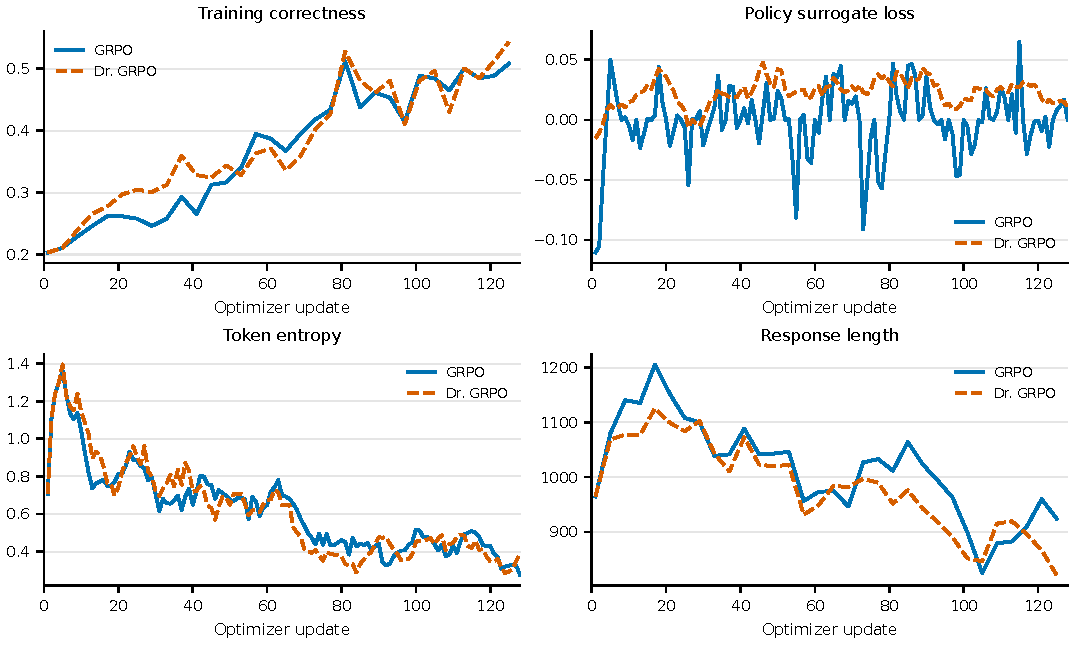
\includegraphics[width=.92\linewidth]{figures/initial_training.pdf}\par\captionof{figure}{Matched initial GRPO and Dr. GRPO runs at learning rate 1e-6: training correctness, surrogate loss, token entropy and response length. Curves summarize observed training updates, not held-out performance.}\end{center}

\begin{center}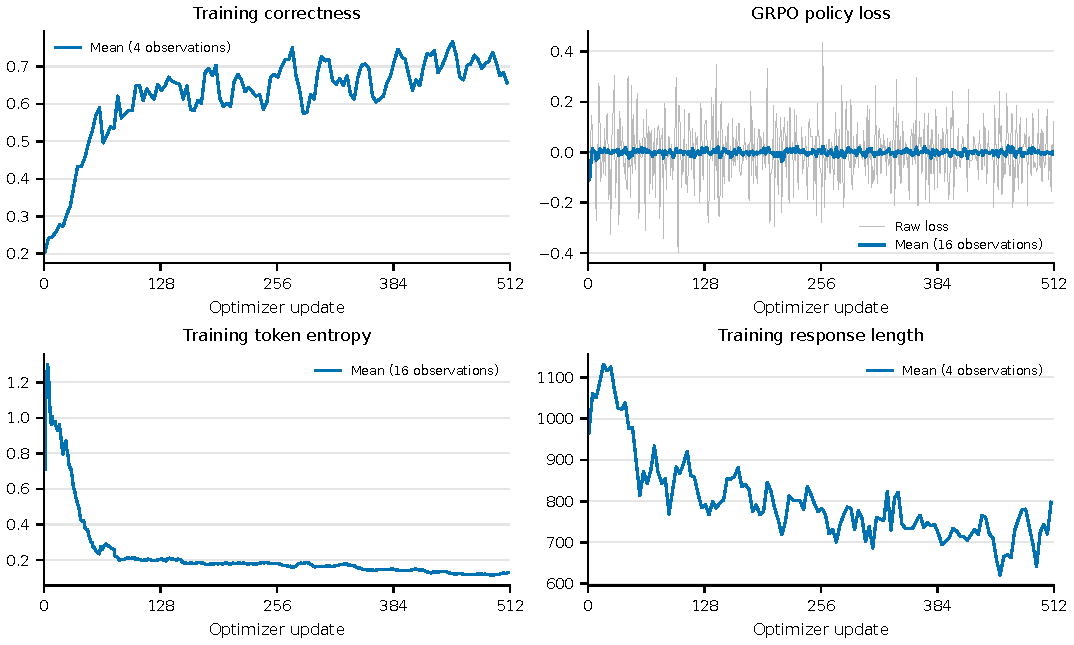
\includegraphics[width=.92\linewidth]{figures/extended_training.pdf}\par\captionof{figure}{Tuned GRPO at learning rate 3e-6 through 512 updates. Pale loss traces are raw observations; darker curves are trailing means. Policy-surrogate loss is not a supervised prediction loss and need not decrease monotonically.}\end{center}

\clearpage

\section{Numerical Training Dynamics}

\begingroup\footnotesize\setlength{\tabcolsep}{3pt}
\begin{longtable}{>{\raggedright\arraybackslash}p{0.2520\linewidth}>{\raggedright\arraybackslash}p{0.1440\linewidth}>{\raggedright\arraybackslash}p{0.1440\linewidth}>{\raggedright\arraybackslash}p{0.1800\linewidth}>{\raggedright\arraybackslash}p{0.1800\linewidth}}
\caption{Policy-surrogate loss: numerical summaries of observed optimizer-update logs.}\\
\toprule Training run & Mean loss & Loss SD & First-quarter mean & Last-quarter mean \\
\midrule\endfirsthead
\toprule Training run & Mean loss & Loss SD & First-quarter mean & Last-quarter mean \\
\midrule\endhead
\midrule\multicolumn{5}{r}{Continued on next page}\endfoot
\bottomrule\endlastfoot
GRPO original & -3.672e-05 & 1.482e-01 & 9.375e-06 & -1.563e-04 \\
Dr. GRPO original & 2.307e-02 & 3.086e-02 & 1.694e-02 & 2.158e-02 \\
DAPO-style original & 1.503e-01 & 1.933e-01 & 1.051e-01 & 1.857e-01 \\
GSPO original & 6.797e-05 & 1.565e-01 & 4.688e-05 & 6.563e-05 \\
Tuned GRPO 128 & -7.344e-05 & 1.375e-01 & -5.000e-05 & 3.125e-06 \\
Tuned GRPO 256 & -3.359e-05 & 1.309e-01 & -4.531e-05 & -6.250e-06 \\
Tuned GRPO 512 & -1.367e-05 & 1.212e-01 & -7.344e-05 & -7.812e-07 \\
\end{longtable}\endgroup


\begingroup\footnotesize\setlength{\tabcolsep}{3pt}
\begin{longtable}{>{\raggedright\arraybackslash}p{0.2248\linewidth}>{\raggedright\arraybackslash}p{0.1079\linewidth}>{\raggedright\arraybackslash}p{0.1079\linewidth}>{\raggedright\arraybackslash}p{0.1079\linewidth}>{\raggedright\arraybackslash}p{0.1169\linewidth}>{\raggedright\arraybackslash}p{0.1169\linewidth}>{\raggedright\arraybackslash}p{0.1169\linewidth}}
\caption{Exploration and response-length dynamics, measured on training generations.}\\
\toprule Training run & Mean entropy & Early entropy & Late entropy & Mean tokens & Early tokens & Late tokens \\
\midrule\endfirsthead
\toprule Training run & Mean entropy & Early entropy & Late entropy & Mean tokens & Early tokens & Late tokens \\
\midrule\endhead
\midrule\multicolumn{7}{r}{Continued on next page}\endfoot
\bottomrule\endlastfoot
GRPO original & 0.599 & 0.864 & 0.406 & 1010 & 1118 & 902 \\
Dr. GRPO original & 0.599 & 0.926 & 0.424 & 974 & 1090 & 868 \\
DAPO-style original & 0.622 & 0.921 & 0.423 & 1005 & 1061 & 929 \\
GSPO original & 0.655 & 0.878 & 0.491 & 1037 & 1053 & 995 \\
Tuned GRPO 128 & 0.379 & 0.783 & 0.202 & 926 & 1080 & 852 \\
Tuned GRPO 256 & 0.281 & 0.549 & 0.182 & 863 & 1002 & 788 \\
Tuned GRPO 512 & 0.213 & 0.379 & 0.129 & 799 & 926 & 718 \\
\end{longtable}\endgroup


\begingroup\footnotesize\setlength{\tabcolsep}{3pt}
\begin{longtable}{>{\raggedright\arraybackslash}p{0.2250\linewidth}>{\raggedright\arraybackslash}p{0.2250\linewidth}>{\raggedright\arraybackslash}p{0.2250\linewidth}>{\raggedright\arraybackslash}p{0.2250\linewidth}}
\caption{Cumulative exposure and training signal during the tuned continuation.}\\
\toprule Updates & Train correctness & Generated M tokens & Mean gradient norm \\
\midrule\endfirsthead
\toprule Updates & Train correctness & Generated M tokens & Mean gradient norm \\
\midrule\endhead
\midrule\multicolumn{4}{r}{Continued on next page}\endfoot
\bottomrule\endlastfoot
128 & 50.15 & 1.897 & 0.628 \\
256 & 57.23 & 3.534 & 0.447 \\
512 & 62.81 & 6.544 & 0.340 \\
\end{longtable}\endgroup


Means use the available observations of each metric through the stated update, excluding step-zero initialization. Early/late values average the first/last quarter of those observations. Loss SD is variation across logged updates, not uncertainty across independent training runs. GRPO and Dr. GRPO use different loss normalization, so their absolute loss and gradient-norm scales are not directly comparable. Continuation rows are nested cumulative prefixes, not independent runs.

\clearpage

\section{Held-Out Trajectories and Exploration}

\begin{center}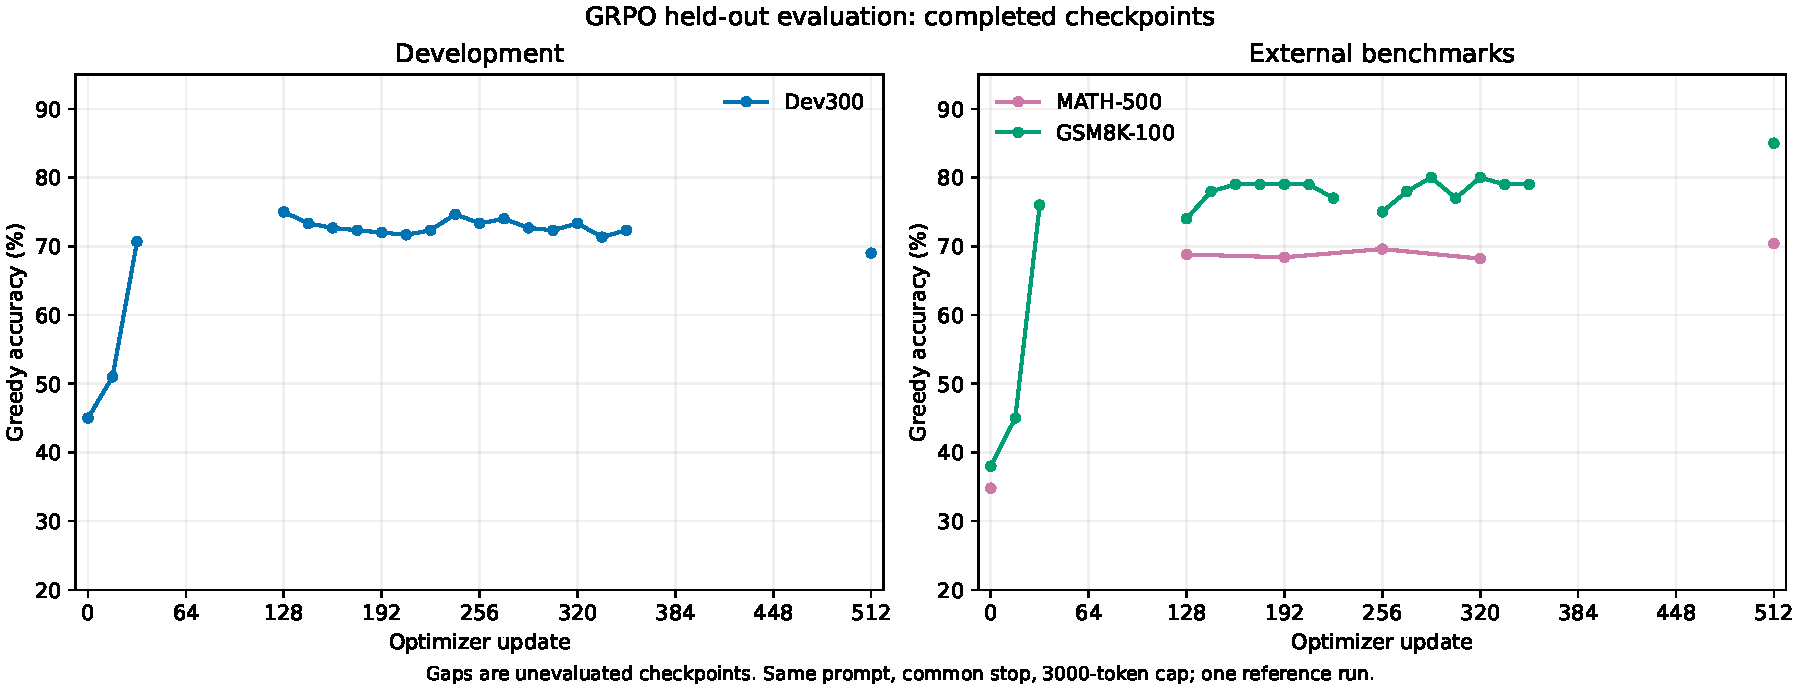
\includegraphics[width=\linewidth]{figures/heldout_accuracy.pdf}\par\captionof{figure}{Measured complete checkpoint cohorts only. Gaps mark unavailable scheduled evaluations; no partial benchmark is scored or interpolated.}\end{center}

\begingroup\footnotesize\setlength{\tabcolsep}{3pt}
\begin{longtable}{>{\raggedright\arraybackslash}p{0.3060\linewidth}>{\raggedright\arraybackslash}p{0.1440\linewidth}>{\raggedright\arraybackslash}p{0.1440\linewidth}>{\raggedright\arraybackslash}p{0.1440\linewidth}>{\raggedright\arraybackslash}p{0.1620\linewidth}}
\caption{Fixed dev100: eight sampled responses at temperature 1; output length is the mean per sampled response.}\\
\toprule Policy & Sampled@1 & Pass@4 & Pass@8 & Response tokens \\
\midrule\endfirsthead
\toprule Policy & Sampled@1 & Pass@4 & Pass@8 & Response tokens \\
\midrule\endhead
\midrule\multicolumn{5}{r}{Continued on next page}\endfoot
\bottomrule\endlastfoot
No RL (original) & 29.38 & 63.87 & 79.00 & 1065 \\
GRPO (original) & 55.00 & 82.79 & 89.00 & 894 \\
Dr. GRPO (original) & 52.62 & 80.97 & 90.00 & 840 \\
DAPO-style (original) & 52.12 & 80.37 & 87.00 & 808 \\
GSPO (original) & 48.25 & 77.97 & 86.00 & 958 \\
Tuned GRPO 128 & 65.50 & 86.20 & 91.00 & 742 \\
Tuned GRPO 256 & 68.00 & 87.71 & 91.00 & 739 \\
Tuned GRPO 512 & 73.25 & 86.77 & 90.00 & 624 \\
\end{longtable}\endgroup


RL changes both the probability of obtaining a correct answer and the distribution of candidate solutions. Oracle pass@8 is consistently higher than sampled@1, leaving room for selection, but availability alone does not establish that voting or a verifier will identify the correct candidate.

\clearpage

\section{Optimizer Ablations}

\begingroup\footnotesize\setlength{\tabcolsep}{3pt}
\begin{longtable}{>{\raggedright\arraybackslash}p{0.1500\linewidth}>{\raggedright\arraybackslash}p{0.1500\linewidth}>{\raggedright\arraybackslash}p{0.1500\linewidth}>{\raggedright\arraybackslash}p{0.1500\linewidth}>{\raggedright\arraybackslash}p{0.1500\linewidth}>{\raggedright\arraybackslash}p{0.1500\linewidth}}
\caption{Learning-rate sweep: dev300 greedy accuracy after 128 updates, fixed reference runs.}\\
\toprule Algorithm & 2e-7 & 5e-7 & 1e-6 & 2e-6 & 3e-6 \\
\midrule\endfirsthead
\toprule Algorithm & 2e-7 & 5e-7 & 1e-6 & 2e-6 & 3e-6 \\
\midrule\endhead
\midrule\multicolumn{6}{r}{Continued on next page}\endfoot
\bottomrule\endlastfoot
GRPO & 49.33 & 61.67 & 72.33 & 70.00 & 75.00 \\
Dr. GRPO & 51.00 & 63.33 & 68.33 & 71.33 & 68.67 \\
DAPO-style & 47.33 & 64.00 & 69.67 & -- & -- \\
GSPO & 48.33 & 63.67 & 70.33 & -- & -- \\
\end{longtable}\endgroup


\begingroup\footnotesize\setlength{\tabcolsep}{3pt}
\begin{longtable}{>{\raggedright\arraybackslash}p{0.1798\linewidth}>{\raggedright\arraybackslash}p{0.1079\linewidth}>{\raggedright\arraybackslash}p{0.1169\linewidth}>{\raggedright\arraybackslash}p{0.1169\linewidth}>{\raggedright\arraybackslash}p{0.1079\linewidth}>{\raggedright\arraybackslash}p{0.1348\linewidth}>{\raggedright\arraybackslash}p{0.1348\linewidth}}
\caption{Learning-rate ablation: measured training behavior, not just final answer accuracy.}\\
\toprule Algorithm & LR & Mean reward & Reward SD & Entropy & Gradient norm & Response tokens \\
\midrule\endfirsthead
\toprule Algorithm & LR & Mean reward & Reward SD & Entropy & Gradient norm & Response tokens \\
\midrule\endhead
\midrule\multicolumn{7}{r}{Continued on next page}\endfoot
\bottomrule\endlastfoot
GRPO & 2e-07 & 0.276 & 0.078 & 0.871 & 1.676 & 1096 \\
GRPO & 5e-07 & 0.280 & 0.095 & 0.813 & 1.502 & 1101 \\
GRPO & 1e-06 & 0.381 & 0.125 & 0.599 & 1.223 & 1010 \\
GRPO & 2e-06 & 0.458 & 0.149 & 0.425 & 0.760 & 945 \\
GRPO & 3e-06 & 0.501 & 0.157 & 0.379 & 0.628 & 926 \\
Dr. GRPO & 2e-07 & 0.270 & 0.078 & 0.866 & 0.066 & 1102 \\
Dr. GRPO & 5e-07 & 0.306 & 0.085 & 0.810 & 0.068 & 1065 \\
Dr. GRPO & 1e-06 & 0.393 & 0.129 & 0.599 & 0.060 & 974 \\
Dr. GRPO & 2e-06 & 0.452 & 0.123 & 0.484 & 0.058 & 943 \\
Dr. GRPO & 3e-06 & 0.511 & 0.157 & 0.364 & 0.049 & 865 \\
DAPO-style & 2e-07 & 0.274 & 0.089 & 0.833 & 0.347 & 1104 \\
DAPO-style & 5e-07 & 0.287 & 0.087 & 0.789 & 0.348 & 1084 \\
DAPO-style & 1e-06 & 0.374 & 0.118 & 0.622 & 0.367 & 1005 \\
GSPO & 2e-07 & 0.260 & 0.088 & 0.869 & 1.255 & 1115 \\
GSPO & 5e-07 & 0.284 & 0.089 & 0.785 & 1.352 & 1090 \\
GSPO & 1e-06 & 0.331 & 0.095 & 0.655 & 1.082 & 1037 \\
\end{longtable}\endgroup


\clearpage

\section{KL and Clipping Ablations}

\begingroup\footnotesize\setlength{\tabcolsep}{3pt}
\begin{longtable}{>{\raggedright\arraybackslash}p{0.1152\linewidth}>{\raggedright\arraybackslash}p{0.0886\linewidth}>{\raggedright\arraybackslash}p{0.1152\linewidth}>{\raggedright\arraybackslash}p{0.1152\linewidth}>{\raggedright\arraybackslash}p{0.1152\linewidth}>{\raggedright\arraybackslash}p{0.1152\linewidth}>{\raggedright\arraybackslash}p{0.1063\linewidth}>{\raggedright\arraybackslash}p{0.1152\linewidth}}
\caption{KL/\allowbreak{}clipping ablation: online KL, offline drift and observed clipping fraction.}\\
\toprule LR & KL beta & Clip bounds & Train KL & Prefix KL & Clip fraction & Entropy & Dev300 \\
\midrule\endfirsthead
\toprule LR & KL beta & Clip bounds & Train KL & Prefix KL & Clip fraction & Entropy & Dev300 \\
\midrule\endhead
\midrule\multicolumn{8}{r}{Continued on next page}\endfoot
\bottomrule\endlastfoot
1e-06 & 0 & 0.2/\allowbreak{}0.2 & -- & 0.0459 & 0.000054 & 0.599 & 72.33 \\
3e-06 & 0 & 0.2/\allowbreak{}0.2 & -- & 0.1063 & 0.000113 & 0.379 & 75.00 \\
1e-06 & 0.001 & 0.2/\allowbreak{}0.2 & 0.00153 & 0.0316 & 0.000048 & 0.655 & 70.33 \\
1e-06 & 0.01 & 0.2/\allowbreak{}0.2 & 0.00184 & 0.0298 & 0.000052 & 0.660 & 71.00 \\
1e-06 & 0 & 0.1/\allowbreak{}0.1 & -- & 0.0229 & 0.002073 & 0.662 & 68.67 \\
1e-06 & 0 & 0.3/\allowbreak{}0.3 & -- & 0.0426 & 0.000007 & 0.619 & 70.67 \\
\end{longtable}\endgroup


GRPO's highest observed development accuracy is at LR 3e-6; Dr. GRPO's is at LR 2e-6. This does not establish a universal ordering: Dr. GRPO exceeds GRPO at LR 2e-6. Prefix KL is an offline shared-context diagnostic, not the online training KL penalty.

\begingroup\footnotesize\setlength{\tabcolsep}{3pt}
\begin{longtable}{>{\raggedright\arraybackslash}p{0.2250\linewidth}>{\raggedright\arraybackslash}p{0.2250\linewidth}>{\raggedright\arraybackslash}p{0.2250\linewidth}>{\raggedright\arraybackslash}p{0.2250\linewidth}}
\caption{External matched-LR comparison at LR 3e-6, 128 updates.}\\
\toprule Method & MATH-500 & GSM8K-100 & AIME-60 \\
\midrule\endfirsthead
\toprule Method & MATH-500 & GSM8K-100 & AIME-60 \\
\midrule\endhead
\midrule\multicolumn{4}{r}{Continued on next page}\endfoot
\bottomrule\endlastfoot
GRPO & 68.80 & 74.00 & 5.00 \\
Dr. GRPO & 67.80 & 80.00 & 5.00 \\
\end{longtable}\endgroup


The Dr. GRPO external row evaluates the matched LR 3e-6 setting, not its development-best LR 2e-6 checkpoint. No unmeasured external score is inferred.

Training reward SD is the source summary's variation across logged reward means; it is not within-group reward variance. Missing online KL means the trainer did not record it, not zero policy drift. Clip fraction is reported as a fraction. Gradient norms depend on each objective's normalization; they should be interpreted within an algorithm.

For GRPO, raising LR from 2e-7 to 3e-6 increases mean training reward from 0.276 to 0.501 while mean entropy falls from 0.871 to 0.379 and mean response length falls from 1,096 to 926 tokens. These measurements show the exploration/optimization trade-off behind the accuracy sweep, rather than only its winning setting.

\clearpage

\section{Reward Design and Training Exploration}

\begingroup\footnotesize\setlength{\tabcolsep}{3pt}
\begin{longtable}{>{\raggedright\arraybackslash}p{0.2880\linewidth}>{\raggedright\arraybackslash}p{0.1350\linewidth}>{\raggedright\arraybackslash}p{0.1530\linewidth}>{\raggedright\arraybackslash}p{0.1710\linewidth}>{\raggedright\arraybackslash}p{0.1530\linewidth}}
\caption{Reward study at LR 3e-6: correctness is logged independently of the shaped reward.}\\
\toprule Reward & Dev300 & Greedy tokens & Train correctness & Train M tokens \\
\midrule\endfirsthead
\toprule Reward & Dev300 & Greedy tokens & Train correctness & Train M tokens \\
\midrule\endhead
\midrule\multicolumn{5}{r}{Continued on next page}\endfoot
\bottomrule\endlastfoot
Correctness only & 75.00 & 722 & 50.15 & 1.90 \\
Correctness + format & 74.00 & 713 & 51.86 & 1.82 \\
Correctness - length & 71.33 & 680 & 36.13 & 1.84 \\
\end{longtable}\endgroup


\begingroup\footnotesize\setlength{\tabcolsep}{3pt}
\begin{longtable}{>{\raggedright\arraybackslash}p{0.2158\linewidth}>{\raggedright\arraybackslash}p{0.1079\linewidth}>{\raggedright\arraybackslash}p{0.1259\linewidth}>{\raggedright\arraybackslash}p{0.1169\linewidth}>{\raggedright\arraybackslash}p{0.0989\linewidth}>{\raggedright\arraybackslash}p{0.1348\linewidth}>{\raggedright\arraybackslash}p{0.0989\linewidth}}
\caption{Reward-design mechanism: raw correctness variance versus shaped-reward variance.}\\
\toprule Reward design & Shaped mean & Correctness variance & Shaped variance & Format \% & Format-only wrong \% & Mean penalty \\
\midrule\endfirsthead
\toprule Reward design & Shaped mean & Correctness variance & Shaped variance & Format \% & Format-only wrong \% & Mean penalty \\
\midrule\endhead
\midrule\multicolumn{7}{r}{Continued on next page}\endfoot
\bottomrule\endlastfoot
Correctness only & 0.5015 & 0.1100 & 0.1100 & -- & 0.00 & 0.00000 \\
+ Format bonus & 0.5989 & 0.1067 & 0.1148 & 80.37 & 30.32 & 0.00000 \\
+ Length penalty & 0.3463 & 0.1267 & 0.1286 & 60.35 & 0.00 & 0.01499 \\
\end{longtable}\endgroup


The format arm adds $0.10F$ to binary correctness $C$; the length arm uses $C-0.05\min(L/3000,1)$. Shaped reward means are not directly comparable across reward definitions. Neither auxiliary reward improves the reference run's development accuracy.

\begingroup\footnotesize\setlength{\tabcolsep}{3pt}
\begin{longtable}{>{\raggedright\arraybackslash}p{0.1500\linewidth}>{\raggedright\arraybackslash}p{0.1500\linewidth}>{\raggedright\arraybackslash}p{0.1500\linewidth}>{\raggedright\arraybackslash}p{0.1500\linewidth}>{\raggedright\arraybackslash}p{0.1500\linewidth}>{\raggedright\arraybackslash}p{0.1500\linewidth}}
\caption{Training temperature/\allowbreak{}group size, evaluated with common inference settings.}\\
\toprule Train T & Group size & Dev300 & Sampled@1 & Pass@8 & Train M tokens \\
\midrule\endfirsthead
\toprule Train T & Group size & Dev300 & Sampled@1 & Pass@8 & Train M tokens \\
\midrule\endhead
\midrule\multicolumn{6}{r}{Continued on next page}\endfoot
\bottomrule\endlastfoot
1 & 4 & 75.00 & 65.50 & 91.00 & 1.90 \\
0.7 & 4 & 73.33 & 64.25 & 90.00 & 1.75 \\
1.3 & 4 & 72.67 & 59.00 & 87.00 & 4.11 \\
1 & 2 & 70.33 & 51.00 & 87.00 & 1.02 \\
1 & 8 & 71.33 & 70.25 & 91.00 & 3.56 \\
\end{longtable}\endgroup


\begingroup\footnotesize\setlength{\tabcolsep}{3pt}
\begin{longtable}{>{\raggedright\arraybackslash}p{0.0797\linewidth}>{\raggedright\arraybackslash}p{0.0886\linewidth}>{\raggedright\arraybackslash}p{0.0886\linewidth}>{\raggedright\arraybackslash}p{0.1063\linewidth}>{\raggedright\arraybackslash}p{0.1240\linewidth}>{\raggedright\arraybackslash}p{0.1418\linewidth}>{\raggedright\arraybackslash}p{0.1418\linewidth}>{\raggedright\arraybackslash}p{0.1152\linewidth}}
\caption{Training-sampling ablation: exposure, reward signal and generated length.}\\
\toprule Train T & Group size & Updates & Responses & Mean tokens & Train correctness & Reward variance & Cost x \\
\midrule\endfirsthead
\toprule Train T & Group size & Updates & Responses & Mean tokens & Train correctness & Reward variance & Cost x \\
\midrule\endhead
\midrule\multicolumn{8}{r}{Continued on next page}\endfoot
\bottomrule\endlastfoot
1 & 4 & 128 & 2048 & 926 & 50.15 & 0.1100 & 1.00 \\
0.7 & 4 & 128 & 2048 & 856 & 60.55 & 0.0996 & 0.92 \\
1.3 & 4 & 128 & 2048 & 2008 & 6.64 & 0.0403 & 2.17 \\
1 & 2 & 64 & 1024 & 998 & 38.77 & 0.0776 & 0.54 \\
1 & 8 & 256 & 4096 & 868 & 55.47 & 0.1202 & 1.87 \\
\end{longtable}\endgroup


Group-size conditions match 512 unique training problems, not optimizer updates or generated tokens: group sizes 2, 4 and 8 use 64, 128 and 256 updates respectively. Higher sampled accuracy can therefore come with substantially different training cost; this is not a compute-matched comparison.

Reward variance is the mean within-prompt variance across generated candidate rewards, not the variance of the reward curve. Cost is generated training tokens relative to the T=1, group-size-4 control; it is not a wall-clock speed ratio. Format-only wrong is the percentage of all training responses that are incorrect yet receive a format bonus.

The format bonus raises mean shaped reward to 0.5989, but 30.32\% of training responses are incorrect and still receive that bonus; higher shaped reward does not imply higher held-out accuracy. Training at T=1.3 generates about 2.17 times the reference tokens while only 6.64\% of sampled training responses are correct. These are sampling-distribution measurements, not greedy evaluation scores.

\clearpage

\section{Supervised and Rejection-Sampling Fine-Tuning}

\begingroup\footnotesize\setlength{\tabcolsep}{3pt}
\begin{longtable}{>{\raggedright\arraybackslash}p{0.2700\linewidth}>{\raggedright\arraybackslash}p{0.1260\linewidth}>{\raggedright\arraybackslash}p{0.1260\linewidth}>{\raggedright\arraybackslash}p{0.1260\linewidth}>{\raggedright\arraybackslash}p{0.1260\linewidth}>{\raggedright\arraybackslash}p{0.1260\linewidth}}
\caption{All independently complete SFT/\allowbreak{}RFT cohorts; unfinished benchmark cohorts are omitted, not prorated.}\\
\toprule Adaptation & Dev300 & MATH-500 & GSM8K-100 & AIME-60 & Dev tokens \\
\midrule\endfirsthead
\toprule Adaptation & Dev300 & MATH-500 & GSM8K-100 & AIME-60 & Dev tokens \\
\midrule\endhead
\midrule\multicolumn{6}{r}{Continued on next page}\endfoot
\bottomrule\endlastfoot
Original full SFT & 40.33 & 47.80 & 70.00 & 1.67 & -- \\
Full SFT & 43.67 & 46.20 & 70.00 & 0.00 & 2178 \\
LoRA SFT & -- & -- & -- & 0.00 & -- \\
Full RFT & 70.67 & 61.80 & 72.00 & 8.33 & 2675 \\
Full RFT, filtered & 70.00 & -- & 75.00 & 6.67 & 2375 \\
LoRA RFT, filtered & -- & -- & 51.00 & 5.00 & -- \\
\end{longtable}\endgroup


SFT imitates human solutions; rejection-sampling fine-tuning (RFT) imitates retained correct model-generated solutions. These use the same source problem pool, but the retained RFT target set is not identical to the human-target training set. Full-parameter follow-ups use LR 5e-6 with a cosine schedule for three epochs; LoRA follow-ups use rank 64, alpha 128 and LR 1e-4. The original SFT control is a separate historical configuration.

\textbf{Interpretation.} RFT improves substantially over human-solution SFT on the complete development and MATH-500 cohorts, but the full RFT MATH-500 score (61.8\%) remains below tuned GRPO. Filtering and parameterization are not uniformly better across available cohorts. Longer RFT responses are not evidence of more efficient reasoning.

\begingroup\footnotesize\setlength{\tabcolsep}{3pt}
\begin{longtable}{>{\raggedright\arraybackslash}p{0.3960\linewidth}>{\raggedright\arraybackslash}p{0.2520\linewidth}>{\raggedright\arraybackslash}p{0.2520\linewidth}}
\caption{Mean completion length on complete external cohorts.}\\
\toprule Adaptation & MATH-500 tokens & GSM8K-100 tokens \\
\midrule\endfirsthead
\toprule Adaptation & MATH-500 tokens & GSM8K-100 tokens \\
\midrule\endhead
\midrule\multicolumn{3}{r}{Continued on next page}\endfoot
\bottomrule\endlastfoot
Original full SFT & 876 & 215 \\
Full SFT & 2207 & 2164 \\
LoRA SFT & -- & -- \\
Full RFT & 2733 & 2659 \\
Full RFT, filtered & -- & 2522 \\
LoRA RFT, filtered & -- & 2625 \\
\end{longtable}\endgroup


The stopping audit confirms that adding the chat-end stop removes truncation in its five-example diagnostic; that diagnostic is a plumbing check, not a benchmark result.

\clearpage

\section{AIME Transfer by Year}

\begingroup\footnotesize\setlength{\tabcolsep}{3pt}
\begin{longtable}{>{\raggedright\arraybackslash}p{0.2250\linewidth}>{\raggedright\arraybackslash}p{0.1350\linewidth}>{\raggedright\arraybackslash}p{0.1350\linewidth}>{\raggedright\arraybackslash}p{0.1350\linewidth}>{\raggedright\arraybackslash}p{0.1350\linewidth}>{\raggedright\arraybackslash}p{0.1350\linewidth}}
\caption{AIME: greedy accuracy and sampled mean@8 /\allowbreak{} oracle pass@8, pooled over both years.}\\
\toprule Policy & 2025 /\allowbreak{}30 & 2026 /\allowbreak{}30 & Pooled /\allowbreak{}60 & Mean@8 & Pass@8 \\
\midrule\endfirsthead
\toprule Policy & 2025 /\allowbreak{}30 & 2026 /\allowbreak{}30 & Pooled /\allowbreak{}60 & Mean@8 & Pass@8 \\
\midrule\endhead
\midrule\multicolumn{6}{r}{Continued on next page}\endfoot
\bottomrule\endlastfoot
No RL & 0.00 & 6.67 & 3.33 & 1.67 & 10.00 \\
GRPO 128 & 0.00 & 10.00 & 5.00 & 3.75 & 15.00 \\
GRPO 256 & 3.33 & 10.00 & 6.67 & 4.17 & 15.00 \\
GRPO 512 & 3.33 & 10.00 & 6.67 & 4.58 & 18.33 \\
\end{longtable}\endgroup


\begingroup\footnotesize\setlength{\tabcolsep}{3pt}
\begin{longtable}{>{\raggedright\arraybackslash}p{0.3000\linewidth}>{\raggedright\arraybackslash}p{0.3000\linewidth}>{\raggedright\arraybackslash}p{0.3000\linewidth}}
\caption{AIME generation behavior on the complete 60-problem greedy cohort.}\\
\toprule Policy & Truncation \% & Mean response tokens \\
\midrule\endfirsthead
\toprule Policy & Truncation \% & Mean response tokens \\
\midrule\endhead
\midrule\multicolumn{3}{r}{Continued on next page}\endfoot
\bottomrule\endlastfoot
No RL & 15.00 & 1397 \\
GRPO 128 & 13.33 & 1295 \\
GRPO 256 & 8.33 & 1144 \\
GRPO 512 & 18.33 & 1309 \\
\end{longtable}\endgroup


AIME remains difficult: pooled greedy gains represent only a few problems, and oracle pass@8 is not a selected-answer score. Small year-specific differences should not be interpreted as reliable algorithm rankings.

\clearpage

\section{Inference Budget and Temperature}

\begingroup\footnotesize\setlength{\tabcolsep}{3pt}
\begin{longtable}{>{\raggedright\arraybackslash}p{0.1800\linewidth}>{\raggedright\arraybackslash}p{0.1800\linewidth}>{\raggedright\arraybackslash}p{0.1800\linewidth}>{\raggedright\arraybackslash}p{0.1800\linewidth}>{\raggedright\arraybackslash}p{0.1800\linewidth}}
\caption{Fixed dev100 greedy accuracy: completion-budget control.}\\
\toprule Policy & 512 tokens & 1,024 & 2,048 & 3,000 \\
\midrule\endfirsthead
\toprule Policy & 512 tokens & 1,024 & 2,048 & 3,000 \\
\midrule\endhead
\midrule\multicolumn{5}{r}{Continued on next page}\endfoot
\bottomrule\endlastfoot
No RL & 28.00 & 48.00 & 50.00 & 50.00 \\
GRPO 128 & 45.00 & 75.00 & 79.00 & 79.00 \\
GRPO 256 & 49.00 & 74.00 & 78.00 & 78.00 \\
GRPO 512 & 50.00 & 71.00 & 74.00 & 74.00 \\
\end{longtable}\endgroup


\begingroup\footnotesize\setlength{\tabcolsep}{3pt}
\begin{longtable}{>{\raggedright\arraybackslash}p{0.1506\linewidth}>{\raggedright\arraybackslash}p{0.0532\linewidth}>{\raggedright\arraybackslash}p{0.0975\linewidth}>{\raggedright\arraybackslash}p{0.1152\linewidth}>{\raggedright\arraybackslash}p{0.1240\linewidth}>{\raggedright\arraybackslash}p{0.1152\linewidth}>{\raggedright\arraybackslash}p{0.1152\linewidth}>{\raggedright\arraybackslash}p{0.1152\linewidth}}
\caption{Inference temperature: voting gains versus the first sampled candidate, missed oracle opportunities and cost.}\\
\toprule Policy & T & Vote \% & Vote gain pp & Missed correct /\allowbreak{}100 & Truncation \% & Response tokens & Group tokens \\
\midrule\endfirsthead
\toprule Policy & T & Vote \% & Vote gain pp & Missed correct /\allowbreak{}100 & Truncation \% & Response tokens & Group tokens \\
\midrule\endhead
\midrule\multicolumn{8}{r}{Continued on next page}\endfoot
\bottomrule\endlastfoot
No RL & 0.4 & 52.00 & +8.0 & 29 & 28.88 & 1364 & 10912 \\
No RL & 0.7 & 44.00 & +6.0 & 41 & 22.38 & 1271 & 10167 \\
No RL & 1.0 & 33.00 & +6.0 & 46 & 10.62 & 1065 & 8518 \\
GRPO 128 & 0.4 & 80.00 & +4.0 & 11 & 2.50 & 683 & 5461 \\
GRPO 128 & 0.7 & 78.00 & +8.0 & 14 & 2.50 & 687 & 5494 \\
GRPO 128 & 1.0 & 73.00 & +11.0 & 18 & 2.38 & 742 & 5933 \\
GRPO 256 & 0.4 & 83.00 & +5.0 & 11 & 2.25 & 670 & 5360 \\
GRPO 256 & 0.7 & 81.00 & +3.0 & 11 & 3.00 & 687 & 5496 \\
GRPO 256 & 1.0 & 71.00 & +9.0 & 20 & 3.88 & 739 & 5911 \\
GRPO 512 & 0.4 & 79.00 & +4.0 & 13 & 2.88 & 618 & 4947 \\
GRPO 512 & 0.7 & 84.00 & +8.0 & 8 & 2.75 & 622 & 4976 \\
GRPO 512 & 1.0 & 79.00 & +1.0 & 11 & 2.12 & 624 & 4994 \\
\end{longtable}\endgroup


A 2,048-token cap matches the 3,000-token cap's aggregate greedy accuracy for all four policies on this dev100 set. This does not prove per-problem equivalence or transfer to longer external problems. Candidate voting can recover correct answers, but requires generating all eight candidates.

\clearpage

\section{Prompt Robustness and External Consensus}

\begingroup\footnotesize\setlength{\tabcolsep}{3pt}
\begin{longtable}{>{\raggedright\arraybackslash}p{0.2250\linewidth}>{\raggedright\arraybackslash}p{0.2250\linewidth}>{\raggedright\arraybackslash}p{0.2250\linewidth}>{\raggedright\arraybackslash}p{0.2250\linewidth}}
\caption{System-instruction sensitivity on fixed dev100, greedy cap 3,000.}\\
\toprule Policy & Original & Reworded & Concise \\
\midrule\endfirsthead
\toprule Policy & Original & Reworded & Concise \\
\midrule\endhead
\midrule\multicolumn{4}{r}{Continued on next page}\endfoot
\bottomrule\endlastfoot
No RL & 50.00 & 40.00 & 32.00 \\
GRPO 128 & 79.00 & 74.00 & 76.00 \\
GRPO 256 & 78.00 & 72.00 & 78.00 \\
GRPO 512 & 74.00 & 80.00 & 77.00 \\
\end{longtable}\endgroup


\begingroup\footnotesize\setlength{\tabcolsep}{3pt}
\begin{longtable}{>{\raggedright\arraybackslash}p{0.1798\linewidth}>{\raggedright\arraybackslash}p{0.1348\linewidth}>{\raggedright\arraybackslash}p{0.1169\linewidth}>{\raggedright\arraybackslash}p{0.1169\linewidth}>{\raggedright\arraybackslash}p{0.0989\linewidth}>{\raggedright\arraybackslash}p{0.0989\linewidth}>{\raggedright\arraybackslash}p{0.1528\linewidth}}
\caption{Complete external consensus: frozen temperature 0.7, eight candidates, original prompt.}\\
\toprule Benchmark & Policy & Greedy & Vote & Fixes* & Breaks* & Token cost x \\
\midrule\endfirsthead
\toprule Benchmark & Policy & Greedy & Vote & Fixes* & Breaks* & Token cost x \\
\midrule\endhead
\midrule\multicolumn{7}{r}{Continued on next page}\endfoot
\bottomrule\endlastfoot
MATH-500 & No RL & 34.80 & 36.60 & 21 & 2 & 6.84 \\
GSM8K-100 & No RL & 38.00 & 38.00 & 1 & 0 & 5.80 \\
GSM8K-100 & GRPO 512 & 85.00 & 86.00 & 4 & 0 & 8.43 \\
MATH-500 & GRPO 512 & 70.40 & 71.20 & 26 & 3 & 7.89 \\
\end{longtable}\endgroup


*Fixes and breaks compare voting against the first sampled candidate, not the greedy control. Token cost is total completion tokens divided by that policy's greedy completion cost. The recovered step512 MATH-500 condition is included only after all 500 problems and eight candidates per problem passed raw-output validation.

Prompt changes affect the no-RL control and RL checkpoints differently. External voting gains are small relative to their completion-token cost: high development oracle accuracy should not be substituted for external selected accuracy.

\clearpage

\section{Candidate Selection and Answer Diversity}

\begingroup\footnotesize\setlength{\tabcolsep}{3pt}
\begin{longtable}{>{\raggedright\arraybackslash}p{0.1798\linewidth}>{\raggedright\arraybackslash}p{0.0539\linewidth}>{\raggedright\arraybackslash}p{0.1259\linewidth}>{\raggedright\arraybackslash}p{0.1259\linewidth}>{\raggedright\arraybackslash}p{0.1259\linewidth}>{\raggedright\arraybackslash}p{0.1438\linewidth}>{\raggedright\arraybackslash}p{0.1438\linewidth}}
\caption{Candidate-budget ablation: marginal gains in percentage points, rather than repeated absolute accuracies.}\\
\toprule Policy & T & Vote 2 gain & Vote 4 gain & Vote 8 gain & Plurality extra 8 & Oracle gap 8 \\
\midrule\endfirsthead
\toprule Policy & T & Vote 2 gain & Vote 4 gain & Vote 8 gain & Plurality extra 8 & Oracle gap 8 \\
\midrule\endhead
\midrule\multicolumn{7}{r}{Continued on next page}\endfoot
\bottomrule\endlastfoot
No RL & 0.4 & +0.00 & +4.45 & +7.50 & +14.58 & 28.25 \\
No RL & 0.7 & +0.00 & +4.40 & +6.88 & +24.87 & 36.88 \\
No RL & 1.0 & +0.00 & +2.66 & +3.88 & +23.25 & 45.75 \\
GRPO 128 & 0.4 & +0.00 & +2.93 & +5.50 & +4.71 & 9.75 \\
GRPO 128 & 0.7 & +0.00 & +4.11 & +6.63 & +4.50 & 13.88 \\
GRPO 128 & 1.0 & +0.00 & +5.39 & +8.62 & +9.13 & 16.88 \\
GRPO 256 & 0.4 & +0.00 & +2.93 & +4.13 & +6.92 & 11.75 \\
GRPO 256 & 0.7 & +0.00 & +3.34 & +5.63 & +6.04 & 10.38 \\
GRPO 256 & 1.0 & +0.00 & +5.59 & +7.75 & +8.21 & 15.25 \\
GRPO 512 & 0.4 & +0.00 & +2.54 & +4.09 & +4.13 & 11.04 \\
GRPO 512 & 0.7 & +0.00 & +3.65 & +7.12 & +2.62 & 9.50 \\
GRPO 512 & 1.0 & +0.00 & +3.60 & +5.36 & +3.71 & 11.39 \\
\end{longtable}\endgroup


These tables reuse saved candidates and average uniformly over subsets and candidate order. They are not new generations or independent replications. In particular, retrospective plurality is a different protocol from the fixed-order strict-majority selector used for external benchmarks. Oracle availability is an upper bound, not a deployable selection rule.

\begingroup\footnotesize\setlength{\tabcolsep}{3pt}
\begin{longtable}{>{\raggedright\arraybackslash}p{0.1500\linewidth}>{\raggedright\arraybackslash}p{0.1500\linewidth}>{\raggedright\arraybackslash}p{0.1500\linewidth}>{\raggedright\arraybackslash}p{0.1500\linewidth}>{\raggedright\arraybackslash}p{0.1500\linewidth}>{\raggedright\arraybackslash}p{0.1500\linewidth}}
\caption{Final-answer diversity (not token-policy entropy), eight candidates per problem.}\\
\toprule Policy & T & Entropy (nats) & Unique answers & Modal mass & Empty \\
\midrule\endfirsthead
\toprule Policy & T & Entropy (nats) & Unique answers & Modal mass & Empty \\
\midrule\endhead
\midrule\multicolumn{6}{r}{Continued on next page}\endfoot
\bottomrule\endlastfoot
No RL & 0.4 & 1.226 & 4.54 & 51.00 & 0.00 \\
No RL & 0.7 & 1.420 & 5.27 & 44.50 & 0.12 \\
No RL & 1 & 1.698 & 6.34 & 32.62 & 0.25 \\
GRPO 128 & 0.4 & 0.521 & 2.46 & 79.25 & 0.00 \\
GRPO 128 & 0.7 & 0.632 & 2.80 & 75.38 & 0.00 \\
GRPO 128 & 1 & 0.797 & 3.31 & 69.25 & 0.00 \\
GRPO 256 & 0.4 & 0.477 & 2.33 & 81.25 & 0.00 \\
GRPO 256 & 0.7 & 0.563 & 2.64 & 78.50 & 0.00 \\
GRPO 256 & 1 & 0.740 & 3.10 & 71.75 & 0.00 \\
GRPO 512 & 0.4 & 0.466 & 2.32 & 81.50 & 0.00 \\
GRPO 512 & 0.7 & 0.510 & 2.45 & 80.00 & 0.00 \\
GRPO 512 & 1 & 0.562 & 2.57 & 77.75 & 0.00 \\
\end{longtable}\endgroup


\clearpage

\section{Selective Coverage and Subgroup Results}

\begingroup\footnotesize\setlength{\tabcolsep}{3pt}
\begin{longtable}{>{\raggedright\arraybackslash}p{0.1708\linewidth}>{\raggedright\arraybackslash}p{0.0539\linewidth}>{\raggedright\arraybackslash}p{0.1259\linewidth}>{\raggedright\arraybackslash}p{0.1259\linewidth}>{\raggedright\arraybackslash}p{0.1259\linewidth}>{\raggedright\arraybackslash}p{0.1438\linewidth}>{\raggedright\arraybackslash}p{0.1528\linewidth}}
\caption{Strict-majority abstention: coverage and accuracy must be reported together.}\\
\toprule Policy & T & Coverage 2 & Coverage 4 & Coverage 8 & Answered acc. 8 & All-problem acc. 8 \\
\midrule\endfirsthead
\toprule Policy & T & Coverage 2 & Coverage 4 & Coverage 8 & Answered acc. 8 & All-problem acc. 8 \\
\midrule\endhead
\midrule\multicolumn{7}{r}{Continued on next page}\endfoot
\bottomrule\endlastfoot
No RL & 0.4 & 31.25 & 36.91 & 41.00 & 92.68 & 38.00 \\
No RL & 0.7 & 23.39 & 27.61 & 30.00 & 93.33 & 28.00 \\
No RL & 1.0 & 12.57 & 14.61 & 15.00 & 93.33 & 14.00 \\
GRPO 128 & 0.4 & 69.89 & 75.16 & 80.00 & 96.25 & 77.00 \\
GRPO 128 & 0.7 & 63.86 & 70.06 & 74.00 & 97.30 & 72.00 \\
GRPO 128 & 1.0 & 54.82 & 63.61 & 69.00 & 95.65 & 66.00 \\
GRPO 256 & 0.4 & 72.29 & 76.54 & 77.00 & 97.24 & 74.88 \\
GRPO 256 & 0.7 & 68.25 & 73.20 & 77.00 & 98.70 & 76.00 \\
GRPO 256 & 1.0 & 57.29 & 66.11 & 68.00 & 98.53 & 67.00 \\
GRPO 512 & 0.4 & 73.36 & 77.76 & 81.00 & 94.71 & 76.71 \\
GRPO 512 & 0.7 & 70.43 & 76.67 & 82.00 & 96.19 & 78.88 \\
GRPO 512 & 1.0 & 67.39 & 72.94 & 76.00 & 97.18 & 73.86 \\
\end{longtable}\endgroup


\begingroup\footnotesize\setlength{\tabcolsep}{3pt}
\begin{longtable}{>{\raggedright\arraybackslash}p{0.2700\linewidth}>{\raggedright\arraybackslash}p{0.0900\linewidth}>{\raggedright\arraybackslash}p{0.1350\linewidth}>{\raggedright\arraybackslash}p{0.1350\linewidth}>{\raggedright\arraybackslash}p{0.1350\linewidth}>{\raggedright\arraybackslash}p{0.1350\linewidth}}
\caption{MATH-500 subgroup behavior: no-RL to GRPO 512, measured on identical complete problem cohorts.}\\
\toprule Subgroup & Gain pp & Base trunc. \% & RL trunc. \% & Base tokens & RL tokens \\
\midrule\endfirsthead
\toprule Subgroup & Gain pp & Base trunc. \% & RL trunc. \% & Base tokens & RL tokens \\
\midrule\endhead
\midrule\multicolumn{6}{r}{Continued on next page}\endfoot
\bottomrule\endlastfoot
Algebra & +53.2 & 54.84 & 1.61 & 1906 & 459 \\
Counting \& Probability & +31.6 & 44.74 & 5.26 & 1662 & 616 \\
Geometry & +29.3 & 31.71 & 4.88 & 1402 & 620 \\
Intermediate Algebra & +16.5 & 21.65 & 7.22 & 1367 & 927 \\
Number Theory & +51.6 & 59.68 & 0.00 & 2022 & 429 \\
Prealgebra & +34.1 & 48.78 & 1.22 & 1681 & 419 \\
Precalculus & +21.4 & 23.21 & 10.71 & 1420 & 1008 \\
Level 1 & +65.1 & 67.44 & 0.00 & 2148 & 299 \\
Level 2 & +43.3 & 58.89 & 0.00 & 1998 & 382 \\
Level 3 & +46.7 & 52.38 & 3.81 & 1870 & 571 \\
Level 4 & +30.5 & 33.59 & 5.47 & 1480 & 681 \\
Level 5 & +17.2 & 21.64 & 6.72 & 1301 & 885 \\
\end{longtable}\endgroup


\clearpage

\section{Grading Sensitivity and General Retention}

\begingroup\footnotesize\setlength{\tabcolsep}{3pt}
\begin{longtable}{>{\raggedright\arraybackslash}p{0.2340\linewidth}>{\raggedright\arraybackslash}p{0.1665\linewidth}>{\raggedright\arraybackslash}p{0.1665\linewidth}>{\raggedright\arraybackslash}p{0.1665\linewidth}>{\raggedright\arraybackslash}p{0.1665\linewidth}}
\caption{Grading audit: each cell is lenient /\allowbreak{} strict closed-box accuracy (November 20 snapshot).}\\
\toprule Policy & Dev300 & MATH-500 & GSM8K-100 & AIME greedy \\
\midrule\endfirsthead
\toprule Policy & Dev300 & MATH-500 & GSM8K-100 & AIME greedy \\
\midrule\endhead
\midrule\multicolumn{5}{r}{Continued on next page}\endfoot
\bottomrule\endlastfoot
No RL & 45.00 /\allowbreak{} 44.67 & 34.80 /\allowbreak{} 33.00 & 38.00 /\allowbreak{} 32.00 & 3.33 /\allowbreak{} 3.33 \\
GRPO original & 72.33 /\allowbreak{} 72.33 & 67.40 /\allowbreak{} 67.20 & 73.00 /\allowbreak{} 73.00 & -- \\
Dr. GRPO original & 68.33 /\allowbreak{} 68.33 & 65.20 /\allowbreak{} 65.20 & 75.00 /\allowbreak{} 75.00 & -- \\
GRPO 128 & 75.00 /\allowbreak{} 74.67 & 68.80 /\allowbreak{} 68.60 & 74.00 /\allowbreak{} 74.00 & 5.00 /\allowbreak{} 5.00 \\
GRPO 256 & 73.33 /\allowbreak{} 73.33 & 69.60 /\allowbreak{} 69.60 & 75.00 /\allowbreak{} 75.00 & 6.67 /\allowbreak{} 6.67 \\
GRPO 512 & 69.00 /\allowbreak{} 68.67 & 70.40 /\allowbreak{} 70.40 & 85.00 /\allowbreak{} 85.00 & 6.67 /\allowbreak{} 6.67 \\
Original full SFT & -- & 47.80 /\allowbreak{} 47.60 & 70.00 /\allowbreak{} 70.00 & -- \\
Full SFT & 43.67 /\allowbreak{} 43.33 & 46.20 /\allowbreak{} 46.60 & 70.00 /\allowbreak{} 68.00 & -- \\
\end{longtable}\endgroup


\begingroup\footnotesize\setlength{\tabcolsep}{3pt}
\begin{longtable}{>{\raggedright\arraybackslash}p{0.1500\linewidth}>{\raggedright\arraybackslash}p{0.1500\linewidth}>{\raggedright\arraybackslash}p{0.1500\linewidth}>{\raggedright\arraybackslash}p{0.1500\linewidth}>{\raggedright\arraybackslash}p{0.1500\linewidth}>{\raggedright\arraybackslash}p{0.1500\linewidth}}
\caption{Original LR 1e-6 policies: auxiliary retention controls.}\\
\toprule Policy & WikiText PPL & BoolQ raw & BoolQ chat & ARC raw & ARC chat \\
\midrule\endfirsthead
\toprule Policy & WikiText PPL & BoolQ raw & BoolQ chat & ARC raw & ARC chat \\
\midrule\endhead
\midrule\multicolumn{6}{r}{Continued on next page}\endfoot
\bottomrule\endlastfoot
No RL & 24.04 & 55.00 & 46.00 & 73.00 & 28.00 \\
GRPO & 24.11 & 54.00 & 47.00 & 73.00 & 42.00 \\
Dr. GRPO & 24.09 & 54.00 & 48.00 & 73.00 & 46.00 \\
DAPO-style & 24.10 & 54.00 & 47.00 & 73.00 & 44.00 \\
GSPO & 24.10 & 54.00 & 46.00 & 73.00 & 32.00 \\
\end{longtable}\endgroup


WikiText perplexity uses 32 fixed 512-token blocks; classification probes use 100 questions each. Raw versus chat formatting changes label likelihoods substantially, so these narrow diagnostics do not establish broad capability preservation. The strict-box audit changes the extraction convention, not historical training rewards, and final-answer correctness is not proof verification.

\clearpage

\section{Paired Improvements and Evidence Scope}

\begingroup\footnotesize\setlength{\tabcolsep}{3pt}
\begin{longtable}{>{\raggedright\arraybackslash}p{0.1440\linewidth}>{\raggedright\arraybackslash}p{0.3330\linewidth}>{\raggedright\arraybackslash}p{0.0810\linewidth}>{\raggedright\arraybackslash}p{0.1800\linewidth}>{\raggedright\arraybackslash}p{0.0810\linewidth}>{\raggedright\arraybackslash}p{0.0810\linewidth}}
\caption{Consolidated final-checkpoint gains: paired bootstrap differences, historical lenient grading.}\\
\toprule Cohort & Comparison & Delta & 95\% CI & Fixed & Broken \\
\midrule\endfirsthead
\toprule Cohort & Comparison & Delta & 95\% CI & Fixed & Broken \\
\midrule\endhead
\midrule\multicolumn{6}{r}{Continued on next page}\endfoot
\bottomrule\endlastfoot
Dev300 & GRPO 512 vs No RL & +24.0 & [+17.7, +30.3] & 92 & 20 \\
MATH-500 & GRPO 512 vs No RL & +35.6 & [+30.6, +40.6] & 201 & 23 \\
GSM8K-100 & GRPO 512 vs No RL & +47.0 & [+36.0, +58.0] & 50 & 3 \\
AIME greedy & GRPO 512 vs No RL & +3.3 & [+0.0, +8.3] & 2 & 0 \\
AIME sampled & GRPO 512 vs No RL & +2.9 & [+0.4, +5.6] & 10 & 2 \\
\end{longtable}\endgroup


Intervals resample paired problems, not training seeds; they do not measure training-run uncertainty and are not corrected for multiple comparisons. Main tables use a fixed reference run rather than selecting favorable seeds. Complete results with worse accuracy remain visible; failed or partial cohorts never receive a score.

The accompanying JSON preserves exact metrics and source hashes. Older unavailable 7B/retrieval outputs are not reconstructed from conversation history. No new training, generation or cluster jobs are needed to build this document.

\clearpage

\section{Learning-Signal Diagnostics}

\begingroup\footnotesize\setlength{\tabcolsep}{3pt}
\begin{longtable}{>{\raggedright\arraybackslash}p{0.2160\linewidth}>{\raggedright\arraybackslash}p{0.1620\linewidth}>{\raggedright\arraybackslash}p{0.1980\linewidth}>{\raggedright\arraybackslash}p{0.1620\linewidth}>{\raggedright\arraybackslash}p{0.1620\linewidth}}
\caption{Original dev100 exploration: distribution of correct candidates across eight sampled solutions.}\\
\toprule Policy & All wrong \% & Mixed correctness \% & All correct \% & Sampled truncation \% \\
\midrule\endfirsthead
\toprule Policy & All wrong \% & Mixed correctness \% & All correct \% & Sampled truncation \% \\
\midrule\endhead
\midrule\multicolumn{5}{r}{Continued on next page}\endfoot
\bottomrule\endlastfoot
No RL & 21.00 & 79.00 & 0.00 & 10.62 \\
GRPO & 11.00 & 80.00 & 9.00 & 7.00 \\
Dr. GRPO & 10.00 & 82.00 & 8.00 & 4.62 \\
DAPO-style & 13.00 & 83.00 & 4.00 & 4.62 \\
GSPO & 14.00 & 77.00 & 9.00 & 8.50 \\
\end{longtable}\endgroup


\begingroup\footnotesize\setlength{\tabcolsep}{3pt}
\begin{longtable}{>{\raggedright\arraybackslash}p{0.1890\linewidth}>{\raggedright\arraybackslash}p{0.1170\linewidth}>{\raggedright\arraybackslash}p{0.1980\linewidth}>{\raggedright\arraybackslash}p{0.1980\linewidth}>{\raggedright\arraybackslash}p{0.1980\linewidth}}
\caption{Training learning signal across all completed learning-rate arms.}\\
\toprule Algorithm & LR & Mean group reward SD & Zero-variance groups \% & Mixed-reward groups \% \\
\midrule\endfirsthead
\toprule Algorithm & LR & Mean group reward SD & Zero-variance groups \% & Mixed-reward groups \% \\
\midrule\endhead
\midrule\multicolumn{5}{r}{Continued on next page}\endfoot
\bottomrule\endlastfoot
GRPO & 2e-07 & 0.2958 & 43.95 & 56.05 \\
GRPO & 5e-07 & 0.3110 & 40.82 & 59.18 \\
GRPO & 1e-06 & 0.3204 & 39.45 & 60.55 \\
GRPO & 2e-06 & 0.3006 & 42.58 & 57.42 \\
GRPO & 3e-06 & 0.2774 & 47.27 & 52.73 \\
Dr. GRPO & 2e-07 & 0.3012 & 42.97 & 57.03 \\
Dr. GRPO & 5e-07 & 0.3221 & 38.67 & 61.33 \\
Dr. GRPO & 1e-06 & 0.3085 & 41.60 & 58.40 \\
Dr. GRPO & 2e-06 & 0.2985 & 43.36 & 56.64 \\
Dr. GRPO & 3e-06 & 0.2691 & 48.63 & 51.37 \\
DAPO-style & 2e-07 & 0.2977 & 43.75 & 56.25 \\
DAPO-style & 5e-07 & 0.2978 & 43.16 & 56.84 \\
DAPO-style & 1e-06 & 0.3248 & 38.48 & 61.52 \\
GSPO & 2e-07 & 0.2839 & 46.09 & 53.91 \\
GSPO & 5e-07 & 0.3016 & 42.58 & 57.42 \\
GSPO & 1e-06 & 0.3227 & 38.87 & 61.13 \\
\end{longtable}\endgroup


The first table describes eight-sample evaluation groups; the second describes training groups, normally four responses per prompt. Mixed means some candidates are correct and others wrong, not a mixture of reward definitions. Zero-variance groups have zero centered reward advantage, but optimizer momentum or an explicit KL term can still change parameters. Group reward SD is not the standard deviation of the training reward curve. DAPO-style here retains the fixed prompt pool rather than dynamically resampling informative groups.

\clearpage

\section{Checkpoint and Restart Validation}

\begingroup\footnotesize\setlength{\tabcolsep}{3pt}
\begin{longtable}{>{\raggedright\arraybackslash}p{0.1800\linewidth}>{\raggedright\arraybackslash}p{0.1800\linewidth}>{\raggedright\arraybackslash}p{0.1350\linewidth}>{\raggedright\arraybackslash}p{0.1710\linewidth}>{\raggedright\arraybackslash}p{0.1170\linewidth}>{\raggedright\arraybackslash}p{0.1170\linewidth}}
\caption{Saved uninterrupted-versus-resumed proof checks, not new benchmark runs.}\\
\toprule Algorithm & Restart /\allowbreak{} final update & Rollouts & Max weight difference & Tolerance & Validation \\
\midrule\endfirsthead
\toprule Algorithm & Restart /\allowbreak{} final update & Rollouts & Max weight difference & Tolerance & Validation \\
\midrule\endhead
\midrule\multicolumn{6}{r}{Continued on next page}\endfoot
\bottomrule\endlastfoot
GRPO & 4 -> 8 & identical & 0.0e+00 & 1.0e-07 & passed \\
Dr. GRPO & 4 -> 8 & identical & 0.0e+00 & 1.0e-07 & passed \\
DAPO-style & 4 -> 8 & identical & 0.0e+00 & 1.0e-07 & passed \\
GSPO & 4 -> 8 & identical & 0.0e+00 & 1.0e-07 & passed \\
Extended GRPO & 8 -> 16 & identical & 0.0e+00 & 1.0e-07 & passed \\
\end{longtable}\endgroup


\begingroup\footnotesize\setlength{\tabcolsep}{3pt}
\begin{longtable}{>{\raggedright\arraybackslash}p{0.1170\linewidth}>{\raggedright\arraybackslash}p{0.1800\linewidth}>{\raggedright\arraybackslash}p{0.1980\linewidth}>{\raggedright\arraybackslash}p{0.4050\linewidth}}
\caption{Reconstructed intermediate checkpoints: narrower rollout/\allowbreak{}metric-prefix evidence.}\\
\toprule Checkpoint & Rollout prefix & Training metric prefix & Original weight-hash equality \\
\midrule\endfirsthead
\toprule Checkpoint & Rollout prefix & Training metric prefix & Original weight-hash equality \\
\midrule\endhead
\midrule\multicolumn{4}{r}{Continued on next page}\endfoot
\bottomrule\endlastfoot
192 & identical & matched & Unavailable: original intermediate weights rotated \\
256 & identical & matched & Unavailable: original intermediate weights rotated \\
\end{longtable}\endgroup


The original four-algorithm gates restart after update 4 and compare at update 8; the extended GRPO gate crosses a repeated-data-pass boundary, restarting at 8 and comparing at 16. Before continuation, the original gates also check checkpoint-boundary equality. Saved proofs require matching sampled completions, parameter keys, deterministic configuration and a maximum weight difference no larger than 1e-7. These are implementation checks, not evidence of better reasoning. Historical failed attempts are not reclassified as passed; only the successful replacement proofs are tabulated.

The reconstructed 192/256 checkpoints match original rollout and logged-training prefixes. Their original intermediate weight files were rotated, so no direct original-weight hash equality is claimed. This weaker reconstruction evidence remains separate from the full restart-equivalence gates.

\clearpage

\section{Supplement: Inference Subgroup Ablations}

All 120 saved category/level breakdowns are shown below. These use the same fixed dev100 problems and eight-candidate, fixed-order strict-majority/first-candidate-fallback inference. They are not MATH-500 subgroup evaluations or retrospective subset/order averages. Voting gain is relative to the first sampled candidate; oracle gap is availability minus selected accuracy, not a deployable gain. Small subgroups have correspondingly coarse percentages.

\begingroup\footnotesize\setlength{\tabcolsep}{3pt}
\begin{longtable}{>{\raggedright\arraybackslash}p{0.2215\linewidth}>{\raggedright\arraybackslash}p{0.1329\linewidth}>{\raggedright\arraybackslash}p{0.0709\linewidth}>{\raggedright\arraybackslash}p{0.0886\linewidth}>{\raggedright\arraybackslash}p{0.0886\linewidth}>{\raggedright\arraybackslash}p{0.1063\linewidth}>{\raggedright\arraybackslash}p{0.0886\linewidth}>{\raggedright\arraybackslash}p{0.0886\linewidth}}
\caption{Category ablation at inference temperature 0.4: complete dev100 subgroup metrics.}\\
\toprule Category & Policy & Problems & Vote \% & Gain pp & Oracle gap pp & Truncation \% & Response tokens \\
\midrule\endfirsthead
\toprule Category & Policy & Problems & Vote \% & Gain pp & Oracle gap pp & Truncation \% & Response tokens \\
\midrule\endhead
\midrule\multicolumn{8}{r}{Continued on next page}\endfoot
\bottomrule\endlastfoot
Algebra & No RL & 15 & 46.67 & +0.0 & 20.0 & 40.83 & 1603 \\
Algebra & GRPO 128 & 15 & 93.33 & +6.7 & 0.0 & 1.67 & 568 \\
Algebra & GRPO 256 & 15 & 86.67 & +0.0 & 13.3 & 3.33 & 591 \\
Algebra & GRPO 512 & 15 & 93.33 & +0.0 & 6.7 & 1.67 & 473 \\
Counting \& Probability & No RL & 15 & 33.33 & +0.0 & 60.0 & 40.83 & 1545 \\
Counting \& Probability & GRPO 128 & 15 & 80.00 & +0.0 & 13.3 & 0.83 & 533 \\
Counting \& Probability & GRPO 256 & 15 & 80.00 & +6.7 & 13.3 & 0.00 & 499 \\
Counting \& Probability & GRPO 512 & 15 & 73.33 & +6.7 & 13.3 & 1.67 & 493 \\
Geometry & No RL & 15 & 60.00 & +13.3 & 6.7 & 14.17 & 1098 \\
Geometry & GRPO 128 & 15 & 73.33 & +13.3 & 0.0 & 2.50 & 881 \\
Geometry & GRPO 256 & 15 & 66.67 & +0.0 & 6.7 & 3.33 & 867 \\
Geometry & GRPO 512 & 15 & 60.00 & +0.0 & 13.3 & 7.50 & 883 \\
Intermediate Algebra & No RL & 15 & 60.00 & +6.7 & 40.0 & 6.67 & 1031 \\
Intermediate Algebra & GRPO 128 & 15 & 66.67 & +6.7 & 33.3 & 6.67 & 1005 \\
Intermediate Algebra & GRPO 256 & 15 & 80.00 & +20.0 & 20.0 & 2.50 & 899 \\
Intermediate Algebra & GRPO 512 & 15 & 73.33 & +13.3 & 26.7 & 5.00 & 908 \\
Number Theory & No RL & 15 & 53.33 & +20.0 & 33.3 & 35.83 & 1442 \\
Number Theory & GRPO 128 & 15 & 80.00 & +0.0 & 20.0 & 4.17 & 583 \\
Number Theory & GRPO 256 & 15 & 80.00 & +6.7 & 20.0 & 4.17 & 638 \\
Number Theory & GRPO 512 & 15 & 86.67 & +6.7 & 13.3 & 2.50 & 527 \\
Prealgebra & No RL & 13 & 61.54 & +7.7 & 15.4 & 39.42 & 1468 \\
Prealgebra & GRPO 128 & 13 & 92.31 & +0.0 & 0.0 & 0.00 & 407 \\
Prealgebra & GRPO 256 & 13 & 100.00 & +0.0 & 0.0 & 0.00 & 400 \\
Prealgebra & GRPO 512 & 13 & 92.31 & +0.0 & 7.7 & 0.00 & 314 \\
Precalculus & No RL & 12 & 50.00 & +8.3 & 25.0 & 25.00 & 1378 \\
Precalculus & GRPO 128 & 12 & 75.00 & +0.0 & 8.3 & 1.04 & 785 \\
Precalculus & GRPO 256 & 12 & 91.67 & +0.0 & 0.0 & 2.08 & 782 \\
Precalculus & GRPO 512 & 12 & 75.00 & +0.0 & 8.3 & 1.04 & 705 \\
\end{longtable}\endgroup


\begingroup\footnotesize\setlength{\tabcolsep}{3pt}
\begin{longtable}{>{\raggedright\arraybackslash}p{0.2215\linewidth}>{\raggedright\arraybackslash}p{0.1329\linewidth}>{\raggedright\arraybackslash}p{0.0709\linewidth}>{\raggedright\arraybackslash}p{0.0886\linewidth}>{\raggedright\arraybackslash}p{0.0886\linewidth}>{\raggedright\arraybackslash}p{0.1063\linewidth}>{\raggedright\arraybackslash}p{0.0886\linewidth}>{\raggedright\arraybackslash}p{0.0886\linewidth}}
\caption{Category ablation at inference temperature 0.7: complete dev100 subgroup metrics.}\\
\toprule Category & Policy & Problems & Vote \% & Gain pp & Oracle gap pp & Truncation \% & Response tokens \\
\midrule\endfirsthead
\toprule Category & Policy & Problems & Vote \% & Gain pp & Oracle gap pp & Truncation \% & Response tokens \\
\midrule\endhead
\midrule\multicolumn{8}{r}{Continued on next page}\endfoot
\bottomrule\endlastfoot
Algebra & No RL & 15 & 26.67 & +0.0 & 46.7 & 27.50 & 1382 \\
Algebra & GRPO 128 & 15 & 86.67 & +6.7 & 6.7 & 0.83 & 559 \\
Algebra & GRPO 256 & 15 & 93.33 & +0.0 & 6.7 & 0.83 & 516 \\
Algebra & GRPO 512 & 15 & 93.33 & +0.0 & 6.7 & 0.83 & 490 \\
Counting \& Probability & No RL & 15 & 33.33 & +0.0 & 53.3 & 29.17 & 1314 \\
Counting \& Probability & GRPO 128 & 15 & 73.33 & +13.3 & 13.3 & 0.83 & 546 \\
Counting \& Probability & GRPO 256 & 15 & 73.33 & +6.7 & 13.3 & 0.83 & 547 \\
Counting \& Probability & GRPO 512 & 15 & 86.67 & +6.7 & 6.7 & 0.83 & 476 \\
Geometry & No RL & 15 & 53.33 & +6.7 & 26.7 & 11.67 & 1085 \\
Geometry & GRPO 128 & 15 & 66.67 & +0.0 & 13.3 & 5.83 & 914 \\
Geometry & GRPO 256 & 15 & 66.67 & +6.7 & 6.7 & 4.17 & 848 \\
Geometry & GRPO 512 & 15 & 60.00 & +6.7 & 13.3 & 5.83 & 858 \\
Intermediate Algebra & No RL & 15 & 46.67 & +0.0 & 46.7 & 18.33 & 1308 \\
Intermediate Algebra & GRPO 128 & 15 & 73.33 & +13.3 & 26.7 & 4.17 & 947 \\
Intermediate Algebra & GRPO 256 & 15 & 80.00 & +6.7 & 20.0 & 8.33 & 1003 \\
Intermediate Algebra & GRPO 512 & 15 & 80.00 & +26.7 & 20.0 & 5.00 & 864 \\
Number Theory & No RL & 15 & 46.67 & +13.3 & 46.7 & 25.83 & 1239 \\
Number Theory & GRPO 128 & 15 & 80.00 & +13.3 & 20.0 & 2.50 & 602 \\
Number Theory & GRPO 256 & 15 & 93.33 & +0.0 & 6.7 & 1.67 & 544 \\
Number Theory & GRPO 512 & 15 & 100.00 & +20.0 & 0.0 & 1.67 & 523 \\
Prealgebra & No RL & 13 & 53.85 & +7.7 & 46.2 & 24.04 & 1203 \\
Prealgebra & GRPO 128 & 13 & 84.62 & +0.0 & 15.4 & 0.96 & 418 \\
Prealgebra & GRPO 256 & 13 & 84.62 & +0.0 & 15.4 & 1.92 & 457 \\
Prealgebra & GRPO 512 & 13 & 92.31 & +0.0 & 0.0 & 0.00 & 318 \\
Precalculus & No RL & 12 & 50.00 & +16.7 & 16.7 & 19.79 & 1377 \\
Precalculus & GRPO 128 & 12 & 83.33 & +8.3 & 0.0 & 2.08 & 811 \\
Precalculus & GRPO 256 & 12 & 75.00 & +0.0 & 8.3 & 3.12 & 907 \\
Precalculus & GRPO 512 & 12 & 75.00 & -8.3 & 8.3 & 5.21 & 824 \\
\end{longtable}\endgroup


\begingroup\footnotesize\setlength{\tabcolsep}{3pt}
\begin{longtable}{>{\raggedright\arraybackslash}p{0.2215\linewidth}>{\raggedright\arraybackslash}p{0.1329\linewidth}>{\raggedright\arraybackslash}p{0.0709\linewidth}>{\raggedright\arraybackslash}p{0.0886\linewidth}>{\raggedright\arraybackslash}p{0.0886\linewidth}>{\raggedright\arraybackslash}p{0.1063\linewidth}>{\raggedright\arraybackslash}p{0.0886\linewidth}>{\raggedright\arraybackslash}p{0.0886\linewidth}}
\caption{Category ablation at inference temperature 1: complete dev100 subgroup metrics.}\\
\toprule Category & Policy & Problems & Vote \% & Gain pp & Oracle gap pp & Truncation \% & Response tokens \\
\midrule\endfirsthead
\toprule Category & Policy & Problems & Vote \% & Gain pp & Oracle gap pp & Truncation \% & Response tokens \\
\midrule\endhead
\midrule\multicolumn{8}{r}{Continued on next page}\endfoot
\bottomrule\endlastfoot
Algebra & No RL & 15 & 26.67 & +0.0 & 53.3 & 13.33 & 1115 \\
Algebra & GRPO 128 & 15 & 93.33 & +0.0 & 6.7 & 0.83 & 580 \\
Algebra & GRPO 256 & 15 & 93.33 & +6.7 & 6.7 & 3.33 & 626 \\
Algebra & GRPO 512 & 15 & 93.33 & +0.0 & 0.0 & 1.67 & 509 \\
Counting \& Probability & No RL & 15 & 6.67 & +0.0 & 60.0 & 8.33 & 989 \\
Counting \& Probability & GRPO 128 & 15 & 73.33 & +13.3 & 20.0 & 0.83 & 592 \\
Counting \& Probability & GRPO 256 & 15 & 60.00 & +0.0 & 33.3 & 3.33 & 629 \\
Counting \& Probability & GRPO 512 & 15 & 73.33 & +0.0 & 13.3 & 0.83 & 468 \\
Geometry & No RL & 15 & 46.67 & +13.3 & 20.0 & 6.67 & 871 \\
Geometry & GRPO 128 & 15 & 53.33 & +0.0 & 13.3 & 1.67 & 867 \\
Geometry & GRPO 256 & 15 & 53.33 & +6.7 & 20.0 & 4.17 & 917 \\
Geometry & GRPO 512 & 15 & 60.00 & +0.0 & 13.3 & 6.67 & 891 \\
Intermediate Algebra & No RL & 15 & 46.67 & +0.0 & 40.0 & 15.83 & 1377 \\
Intermediate Algebra & GRPO 128 & 15 & 66.67 & +13.3 & 33.3 & 5.83 & 1091 \\
Intermediate Algebra & GRPO 256 & 15 & 46.67 & +13.3 & 46.7 & 6.67 & 994 \\
Intermediate Algebra & GRPO 512 & 15 & 73.33 & +13.3 & 20.0 & 3.33 & 876 \\
Number Theory & No RL & 15 & 33.33 & +6.7 & 53.3 & 11.67 & 1074 \\
Number Theory & GRPO 128 & 15 & 93.33 & +26.7 & 6.7 & 3.33 & 655 \\
Number Theory & GRPO 256 & 15 & 86.67 & +13.3 & 13.3 & 2.50 & 618 \\
Number Theory & GRPO 512 & 15 & 93.33 & +0.0 & 6.7 & 0.00 & 503 \\
Prealgebra & No RL & 13 & 46.15 & +15.4 & 46.2 & 9.62 & 934 \\
Prealgebra & GRPO 128 & 13 & 84.62 & +7.7 & 7.7 & 0.96 & 519 \\
Prealgebra & GRPO 256 & 13 & 92.31 & +7.7 & 0.0 & 2.88 & 503 \\
Prealgebra & GRPO 512 & 13 & 92.31 & +0.0 & 7.7 & 0.00 & 314 \\
Precalculus & No RL & 12 & 25.00 & +8.3 & 50.0 & 8.33 & 1078 \\
Precalculus & GRPO 128 & 12 & 41.67 & +16.7 & 41.7 & 3.12 & 887 \\
Precalculus & GRPO 256 & 12 & 66.67 & +16.7 & 16.7 & 4.17 & 885 \\
Precalculus & GRPO 512 & 12 & 66.67 & -8.3 & 16.7 & 2.08 & 803 \\
\end{longtable}\endgroup


\begingroup\footnotesize\setlength{\tabcolsep}{3pt}
\begin{longtable}{>{\raggedright\arraybackslash}p{0.2215\linewidth}>{\raggedright\arraybackslash}p{0.1329\linewidth}>{\raggedright\arraybackslash}p{0.0709\linewidth}>{\raggedright\arraybackslash}p{0.0886\linewidth}>{\raggedright\arraybackslash}p{0.0886\linewidth}>{\raggedright\arraybackslash}p{0.1063\linewidth}>{\raggedright\arraybackslash}p{0.0886\linewidth}>{\raggedright\arraybackslash}p{0.0886\linewidth}}
\caption{Difficulty ablation at inference temperature 0.4: complete dev100 subgroup metrics.}\\
\toprule Difficulty & Policy & Problems & Vote \% & Gain pp & Oracle gap pp & Truncation \% & Response tokens \\
\midrule\endfirsthead
\toprule Difficulty & Policy & Problems & Vote \% & Gain pp & Oracle gap pp & Truncation \% & Response tokens \\
\midrule\endhead
\midrule\multicolumn{8}{r}{Continued on next page}\endfoot
\bottomrule\endlastfoot
Level 3 & No RL & 34 & 64.71 & +5.9 & 17.6 & 39.71 & 1522 \\
Level 3 & GRPO 128 & 34 & 97.06 & +2.9 & 2.9 & 0.00 & 494 \\
Level 3 & GRPO 256 & 34 & 100.00 & +2.9 & 0.0 & 0.37 & 489 \\
Level 3 & GRPO 512 & 34 & 100.00 & +0.0 & 0.0 & 0.00 & 407 \\
Level 4 & No RL & 33 & 48.48 & +6.1 & 39.4 & 31.44 & 1403 \\
Level 4 & GRPO 128 & 33 & 72.73 & +3.0 & 18.2 & 2.65 & 679 \\
Level 4 & GRPO 256 & 33 & 78.79 & +9.1 & 15.2 & 3.41 & 695 \\
Level 4 & GRPO 512 & 33 & 75.76 & +12.1 & 18.2 & 4.17 & 628 \\
Level 5 & No RL & 33 & 42.42 & +12.1 & 30.3 & 15.15 & 1162 \\
Level 5 & GRPO 128 & 33 & 69.70 & +6.1 & 12.1 & 4.92 & 880 \\
Level 5 & GRPO 256 & 33 & 69.70 & +3.0 & 18.2 & 3.03 & 831 \\
Level 5 & GRPO 512 & 33 & 60.61 & +0.0 & 21.2 & 4.55 & 826 \\
\end{longtable}\endgroup


\begingroup\footnotesize\setlength{\tabcolsep}{3pt}
\begin{longtable}{>{\raggedright\arraybackslash}p{0.2215\linewidth}>{\raggedright\arraybackslash}p{0.1329\linewidth}>{\raggedright\arraybackslash}p{0.0709\linewidth}>{\raggedright\arraybackslash}p{0.0886\linewidth}>{\raggedright\arraybackslash}p{0.0886\linewidth}>{\raggedright\arraybackslash}p{0.1063\linewidth}>{\raggedright\arraybackslash}p{0.0886\linewidth}>{\raggedright\arraybackslash}p{0.0886\linewidth}}
\caption{Difficulty ablation at inference temperature 0.7: complete dev100 subgroup metrics.}\\
\toprule Difficulty & Policy & Problems & Vote \% & Gain pp & Oracle gap pp & Truncation \% & Response tokens \\
\midrule\endfirsthead
\toprule Difficulty & Policy & Problems & Vote \% & Gain pp & Oracle gap pp & Truncation \% & Response tokens \\
\midrule\endhead
\midrule\multicolumn{8}{r}{Continued on next page}\endfoot
\bottomrule\endlastfoot
Level 3 & No RL & 34 & 44.12 & +0.0 & 47.1 & 27.94 & 1325 \\
Level 3 & GRPO 128 & 34 & 97.06 & +5.9 & 2.9 & 0.37 & 494 \\
Level 3 & GRPO 256 & 34 & 100.00 & +2.9 & 0.0 & 0.74 & 504 \\
Level 3 & GRPO 512 & 34 & 100.00 & +2.9 & 0.0 & 0.37 & 412 \\
Level 4 & No RL & 33 & 39.39 & +3.0 & 42.4 & 22.73 & 1304 \\
Level 4 & GRPO 128 & 33 & 78.79 & +12.1 & 15.2 & 3.79 & 685 \\
Level 4 & GRPO 256 & 33 & 78.79 & +3.0 & 15.2 & 1.89 & 653 \\
Level 4 & GRPO 512 & 33 & 81.82 & +12.1 & 12.1 & 3.79 & 621 \\
Level 5 & No RL & 33 & 48.48 & +15.2 & 33.3 & 16.29 & 1183 \\
Level 5 & GRPO 128 & 33 & 57.58 & +6.1 & 24.2 & 3.41 & 887 \\
Level 5 & GRPO 256 & 33 & 63.64 & +3.0 & 18.2 & 6.44 & 910 \\
Level 5 & GRPO 512 & 33 & 69.70 & +9.1 & 12.1 & 4.17 & 840 \\
\end{longtable}\endgroup


\begingroup\footnotesize\setlength{\tabcolsep}{3pt}
\begin{longtable}{>{\raggedright\arraybackslash}p{0.2215\linewidth}>{\raggedright\arraybackslash}p{0.1329\linewidth}>{\raggedright\arraybackslash}p{0.0709\linewidth}>{\raggedright\arraybackslash}p{0.0886\linewidth}>{\raggedright\arraybackslash}p{0.0886\linewidth}>{\raggedright\arraybackslash}p{0.1063\linewidth}>{\raggedright\arraybackslash}p{0.0886\linewidth}>{\raggedright\arraybackslash}p{0.0886\linewidth}}
\caption{Difficulty ablation at inference temperature 1: complete dev100 subgroup metrics.}\\
\toprule Difficulty & Policy & Problems & Vote \% & Gain pp & Oracle gap pp & Truncation \% & Response tokens \\
\midrule\endfirsthead
\toprule Difficulty & Policy & Problems & Vote \% & Gain pp & Oracle gap pp & Truncation \% & Response tokens \\
\midrule\endhead
\midrule\multicolumn{8}{r}{Continued on next page}\endfoot
\bottomrule\endlastfoot
Level 3 & No RL & 34 & 29.41 & +5.9 & 58.8 & 10.29 & 987 \\
Level 3 & GRPO 128 & 34 & 94.12 & +11.8 & 5.9 & 0.37 & 552 \\
Level 3 & GRPO 256 & 34 & 91.18 & +2.9 & 8.8 & 1.47 & 543 \\
Level 3 & GRPO 512 & 34 & 100.00 & +0.0 & 0.0 & 0.37 & 418 \\
Level 4 & No RL & 33 & 30.30 & +6.1 & 51.5 & 10.23 & 1073 \\
Level 4 & GRPO 128 & 33 & 69.70 & +18.2 & 21.2 & 1.14 & 674 \\
Level 4 & GRPO 256 & 33 & 63.64 & +18.2 & 27.3 & 3.79 & 715 \\
Level 4 & GRPO 512 & 33 & 75.76 & -3.0 & 12.1 & 1.89 & 639 \\
Level 5 & No RL & 33 & 39.39 & +6.1 & 27.3 & 11.36 & 1136 \\
Level 5 & GRPO 128 & 33 & 54.55 & +3.0 & 27.3 & 5.68 & 1004 \\
Level 5 & GRPO 256 & 33 & 57.58 & +6.1 & 24.2 & 6.44 & 965 \\
Level 5 & GRPO 512 & 33 & 60.61 & +6.1 & 21.2 & 4.17 & 822 \\
\end{longtable}\endgroup


\clearpage

\section{Supplement: Extraction and Grading Diagnostics}

The following 14 tables cover all 123 independently complete response-level audit groups in the November 20 snapshot. Denominators count responses: a 100-question, eight-sample run contributes 800, not 100. Strict correct requires the audit's closed-box extraction; lenient-only counts accepted answers that strict extraction rejects. Multi-box means multiple distinct boxed answers, not all malformed outputs. Truncation percentages are per response. Stored mismatches compare historical labels to the audit's re-extracted lenient labels and do not silently replace training rewards.

\begingroup\footnotesize\setlength{\tabcolsep}{3pt}
\begin{longtable}{>{\raggedright\arraybackslash}p{0.2835\linewidth}>{\raggedright\arraybackslash}p{0.0886\linewidth}>{\raggedright\arraybackslash}p{0.0886\linewidth}>{\raggedright\arraybackslash}p{0.0797\linewidth}>{\raggedright\arraybackslash}p{0.0797\linewidth}>{\raggedright\arraybackslash}p{0.0975\linewidth}>{\raggedright\arraybackslash}p{0.0797\linewidth}>{\raggedright\arraybackslash}p{0.0886\linewidth}}
\caption{AIME checkpoints: response-level extraction audit.}\\
\toprule Policy /\allowbreak{} protocol & Responses & Strict correct & Lenient only & Trunc. \% & Trunc. strict correct & Multi-box & Stored mismatch \\
\midrule\endfirsthead
\toprule Policy /\allowbreak{} protocol & Responses & Strict correct & Lenient only & Trunc. \% & Trunc. strict correct & Multi-box & Stored mismatch \\
\midrule\endhead
\midrule\multicolumn{8}{r}{Continued on next page}\endfoot
\bottomrule\endlastfoot
No RL /\allowbreak{} greedy & 60 & 2 & 0 & 15.00 & 0 & 1 & 0 \\
No RL /\allowbreak{} sampled & 480 & 8 & 0 & 11.88 & 0 & 78 & 0 \\
GRPO 128 /\allowbreak{} greedy & 60 & 3 & 0 & 13.33 & 0 & 0 & 0 \\
GRPO 128 /\allowbreak{} sampled & 480 & 18 & 0 & 6.67 & 0 & 19 & 0 \\
GRPO 256 /\allowbreak{} greedy & 60 & 4 & 0 & 8.33 & 0 & 0 & 0 \\
GRPO 256 /\allowbreak{} sampled & 480 & 20 & 0 & 6.25 & 0 & 11 & 0 \\
GRPO 512 /\allowbreak{} greedy & 60 & 4 & 0 & 18.33 & 0 & 0 & 0 \\
GRPO 512 /\allowbreak{} sampled & 480 & 22 & 0 & 9.38 & 0 & 6 & 0 \\
\end{longtable}\endgroup


\begingroup\footnotesize\setlength{\tabcolsep}{3pt}
\begin{longtable}{>{\raggedright\arraybackslash}p{0.2835\linewidth}>{\raggedright\arraybackslash}p{0.0886\linewidth}>{\raggedright\arraybackslash}p{0.0886\linewidth}>{\raggedright\arraybackslash}p{0.0797\linewidth}>{\raggedright\arraybackslash}p{0.0797\linewidth}>{\raggedright\arraybackslash}p{0.0975\linewidth}>{\raggedright\arraybackslash}p{0.0797\linewidth}>{\raggedright\arraybackslash}p{0.0886\linewidth}}
\caption{Inference temperature and completion budget: response-level extraction audit.}\\
\toprule Policy /\allowbreak{} protocol & Responses & Strict correct & Lenient only & Trunc. \% & Trunc. strict correct & Multi-box & Stored mismatch \\
\midrule\endfirsthead
\toprule Policy /\allowbreak{} protocol & Responses & Strict correct & Lenient only & Trunc. \% & Trunc. strict correct & Multi-box & Stored mismatch \\
\midrule\endhead
\midrule\multicolumn{8}{r}{Continued on next page}\endfoot
\bottomrule\endlastfoot
No RL greedy T=0 cap=1024 & 100 & 47 & 1 & 35.00 & 2 & 0 & 0 \\
No RL greedy T=0 cap=2048 & 100 & 49 & 1 & 29.00 & 1 & 0 & 0 \\
No RL greedy T=0 cap=512 & 100 & 23 & 5 & 68.00 & 1 & 0 & 0 \\
No RL sampled T=0.4 cap=3000 & 800 & 351 & 12 & 28.88 & 4 & 37 & 1 \\
No RL sampled T=0.7 cap=3000 & 800 & 325 & 8 & 22.38 & 4 & 111 & 3 \\
GRPO 128 greedy T=0 cap=1024 & 100 & 75 & 0 & 11.00 & 0 & 1 & 0 \\
GRPO 128 greedy T=0 cap=2048 & 100 & 78 & 1 & 3.00 & 0 & 1 & 0 \\
GRPO 128 greedy T=0 cap=512 & 100 & 43 & 2 & 56.00 & 1 & 0 & 0 \\
GRPO 128 sampled T=0.4 cap=3000 & 800 & 605 & 1 & 2.50 & 0 & 3 & 0 \\
GRPO 128 sampled T=0.7 cap=3000 & 800 & 573 & 0 & 2.50 & 1 & 10 & 1 \\
GRPO 256 greedy T=0 cap=1024 & 100 & 74 & 0 & 12.00 & 0 & 0 & 0 \\
GRPO 256 greedy T=0 cap=2048 & 100 & 78 & 0 & 5.00 & 0 & 0 & 0 \\
GRPO 256 greedy T=0 cap=512 & 100 & 46 & 3 & 52.00 & 3 & 0 & 0 \\
GRPO 256 sampled T=0.4 cap=3000 & 800 & 625 & 0 & 2.25 & 0 & 7 & 0 \\
GRPO 256 sampled T=0.7 cap=3000 & 800 & 607 & 1 & 3.00 & 0 & 9 & 0 \\
GRPO 512 greedy T=0 cap=1024 & 100 & 71 & 0 & 13.00 & 0 & 2 & 0 \\
GRPO 512 greedy T=0 cap=2048 & 100 & 74 & 0 & 2.00 & 0 & 2 & 0 \\
GRPO 512 greedy T=0 cap=512 & 100 & 50 & 0 & 39.00 & 0 & 1 & 0 \\
GRPO 512 sampled T=0.4 cap=3000 & 800 & 615 & 0 & 2.88 & 0 & 10 & 0 \\
GRPO 512 sampled T=0.7 cap=3000 & 800 & 603 & 0 & 2.75 & 0 & 9 & 0 \\
\end{longtable}\endgroup


\begingroup\footnotesize\setlength{\tabcolsep}{3pt}
\begin{longtable}{>{\raggedright\arraybackslash}p{0.2835\linewidth}>{\raggedright\arraybackslash}p{0.0886\linewidth}>{\raggedright\arraybackslash}p{0.0886\linewidth}>{\raggedright\arraybackslash}p{0.0797\linewidth}>{\raggedright\arraybackslash}p{0.0797\linewidth}>{\raggedright\arraybackslash}p{0.0975\linewidth}>{\raggedright\arraybackslash}p{0.0797\linewidth}>{\raggedright\arraybackslash}p{0.0886\linewidth}}
\caption{External checkpoint benchmarks: response-level extraction audit.}\\
\toprule Policy /\allowbreak{} protocol & Responses & Strict correct & Lenient only & Trunc. \% & Trunc. strict correct & Multi-box & Stored mismatch \\
\midrule\endfirsthead
\toprule Policy /\allowbreak{} protocol & Responses & Strict correct & Lenient only & Trunc. \% & Trunc. strict correct & Multi-box & Stored mismatch \\
\midrule\endhead
\midrule\multicolumn{8}{r}{Continued on next page}\endfoot
\bottomrule\endlastfoot
GRPO 192 /\allowbreak{} Dev100 & 100 & 77 & 0 & 2.00 & 0 & 1 & 0 \\
GRPO 128 /\allowbreak{} GSM8K-100 & 100 & 74 & 0 & 1.00 & 0 & 0 & 0 \\
GRPO 128 /\allowbreak{} MATH-500 & 500 & 343 & 1 & 2.80 & 0 & 0 & 0 \\
GRPO 256 /\allowbreak{} GSM8K-100 & 100 & 75 & 0 & 3.00 & 0 & 0 & 0 \\
GRPO 256 /\allowbreak{} MATH-500 & 500 & 348 & 0 & 3.40 & 0 & 0 & 0 \\
GRPO 512 /\allowbreak{} GSM8K-100 & 100 & 85 & 0 & 0.00 & 0 & 0 & 0 \\
GRPO 512 /\allowbreak{} MATH-500 & 500 & 352 & 0 & 4.00 & 0 & 1 & 0 \\
\end{longtable}\endgroup


\begingroup\footnotesize\setlength{\tabcolsep}{3pt}
\begin{longtable}{>{\raggedright\arraybackslash}p{0.2835\linewidth}>{\raggedright\arraybackslash}p{0.0886\linewidth}>{\raggedright\arraybackslash}p{0.0886\linewidth}>{\raggedright\arraybackslash}p{0.0797\linewidth}>{\raggedright\arraybackslash}p{0.0797\linewidth}>{\raggedright\arraybackslash}p{0.0975\linewidth}>{\raggedright\arraybackslash}p{0.0797\linewidth}>{\raggedright\arraybackslash}p{0.0886\linewidth}}
\caption{Prompt and external consensus follow-ups: response-level extraction audit.}\\
\toprule Policy /\allowbreak{} protocol & Responses & Strict correct & Lenient only & Trunc. \% & Trunc. strict correct & Multi-box & Stored mismatch \\
\midrule\endfirsthead
\toprule Policy /\allowbreak{} protocol & Responses & Strict correct & Lenient only & Trunc. \% & Trunc. strict correct & Multi-box & Stored mismatch \\
\midrule\endhead
\midrule\multicolumn{8}{r}{Continued on next page}\endfoot
\bottomrule\endlastfoot
No RL Dev100 concise prompt greedy & 100 & 32 & 0 & 50.00 & 1 & 1 & 0 \\
No RL Dev100 reworded prompt greedy & 100 & 38 & 1 & 43.00 & 2 & 3 & 1 \\
No RL GSM8K-100 original prompt sampled & 800 & 242 & 41 & 28.75 & 11 & 75 & 3 \\
No RL MATH-500 original prompt sampled & 4000 & 1193 & 68 & 28.32 & 21 & 477 & 4 \\
GRPO 128 Dev100 concise prompt greedy & 100 & 76 & 0 & 2.00 & 0 & 0 & 0 \\
GRPO 128 Dev100 reworded prompt greedy & 100 & 74 & 0 & 3.00 & 0 & 0 & 0 \\
GRPO 256 Dev100 concise prompt greedy & 100 & 78 & 0 & 1.00 & 0 & 0 & 0 \\
GRPO 256 Dev100 reworded prompt greedy & 100 & 72 & 0 & 4.00 & 0 & 0 & 0 \\
GRPO 512 Dev100 concise prompt greedy & 100 & 77 & 0 & 3.00 & 0 & 0 & 0 \\
GRPO 512 Dev100 reworded prompt greedy & 100 & 80 & 0 & 3.00 & 0 & 2 & 0 \\
GRPO 512 GSM8K-100 original prompt sampled & 800 & 630 & 0 & 0.62 & 0 & 4 & 0 \\
GRPO 512 MATH-500 original prompt sampled & 4000 & 2720 & 3 & 3.08 & 0 & 24 & 3 \\
\end{longtable}\endgroup


\begingroup\footnotesize\setlength{\tabcolsep}{3pt}
\begin{longtable}{>{\raggedright\arraybackslash}p{0.2835\linewidth}>{\raggedright\arraybackslash}p{0.0886\linewidth}>{\raggedright\arraybackslash}p{0.0886\linewidth}>{\raggedright\arraybackslash}p{0.0797\linewidth}>{\raggedright\arraybackslash}p{0.0797\linewidth}>{\raggedright\arraybackslash}p{0.0975\linewidth}>{\raggedright\arraybackslash}p{0.0797\linewidth}>{\raggedright\arraybackslash}p{0.0886\linewidth}}
\caption{Common-stop original controls: response-level extraction audit.}\\
\toprule Policy /\allowbreak{} protocol & Responses & Strict correct & Lenient only & Trunc. \% & Trunc. strict correct & Multi-box & Stored mismatch \\
\midrule\endfirsthead
\toprule Policy /\allowbreak{} protocol & Responses & Strict correct & Lenient only & Trunc. \% & Trunc. strict correct & Multi-box & Stored mismatch \\
\midrule\endhead
\midrule\multicolumn{8}{r}{Continued on next page}\endfoot
\bottomrule\endlastfoot
No RL /\allowbreak{} greedy & 300 & 134 & 1 & 31.67 & 1 & 0 & 0 \\
DAPO-style /\allowbreak{} greedy & 300 & 209 & 0 & 2.67 & 0 & 1 & 0 \\
Dr. GRPO /\allowbreak{} greedy & 300 & 205 & 0 & 1.33 & 0 & 1 & 0 \\
GRPO /\allowbreak{} greedy & 300 & 217 & 0 & 2.33 & 0 & 1 & 0 \\
GSPO /\allowbreak{} greedy & 300 & 211 & 0 & 1.67 & 0 & 1 & 0 \\
SFT /\allowbreak{} greedy & 300 & 121 & 0 & 23.67 & 18 & 7 & 0 \\
No RL /\allowbreak{} sampled & 800 & 229 & 9 & 10.62 & 3 & 149 & 3 \\
DAPO-style /\allowbreak{} sampled & 800 & 419 & 2 & 4.62 & 4 & 67 & 4 \\
Dr. GRPO /\allowbreak{} sampled & 800 & 421 & 1 & 4.62 & 2 & 69 & 1 \\
GRPO /\allowbreak{} sampled & 800 & 439 & 2 & 7.00 & 3 & 94 & 1 \\
GSPO /\allowbreak{} sampled & 800 & 384 & 2 & 8.50 & 1 & 105 & 0 \\
\end{longtable}\endgroup


\begingroup\footnotesize\setlength{\tabcolsep}{3pt}
\begin{longtable}{>{\raggedright\arraybackslash}p{0.2835\linewidth}>{\raggedright\arraybackslash}p{0.0886\linewidth}>{\raggedright\arraybackslash}p{0.0886\linewidth}>{\raggedright\arraybackslash}p{0.0797\linewidth}>{\raggedright\arraybackslash}p{0.0797\linewidth}>{\raggedright\arraybackslash}p{0.0975\linewidth}>{\raggedright\arraybackslash}p{0.0797\linewidth}>{\raggedright\arraybackslash}p{0.0886\linewidth}}
\caption{Intermediate checkpoint evaluations: response-level extraction audit.}\\
\toprule Policy /\allowbreak{} protocol & Responses & Strict correct & Lenient only & Trunc. \% & Trunc. strict correct & Multi-box & Stored mismatch \\
\midrule\endfirsthead
\toprule Policy /\allowbreak{} protocol & Responses & Strict correct & Lenient only & Trunc. \% & Trunc. strict correct & Multi-box & Stored mismatch \\
\midrule\endhead
\midrule\multicolumn{8}{r}{Continued on next page}\endfoot
\bottomrule\endlastfoot
GRPO 144 /\allowbreak{} Dev300 & 300 & 220 & 0 & 4.33 & 0 & 1 & 0 \\
GRPO 144 /\allowbreak{} GSM8K-100 & 100 & 78 & 0 & 1.00 & 0 & 0 & 0 \\
GRPO 160 /\allowbreak{} Dev300 & 300 & 218 & 0 & 5.00 & 1 & 1 & 0 \\
GRPO 160 /\allowbreak{} GSM8K-100 & 100 & 79 & 0 & 1.00 & 0 & 0 & 0 \\
GRPO 176 /\allowbreak{} Dev300 & 300 & 217 & 0 & 4.00 & 0 & 1 & 0 \\
GRPO 176 /\allowbreak{} GSM8K-100 & 100 & 79 & 0 & 1.00 & 0 & 0 & 0 \\
GRPO 272 /\allowbreak{} Dev300 & 300 & 222 & 0 & 4.67 & 0 & 1 & 0 \\
GRPO 272 /\allowbreak{} GSM8K-100 & 100 & 78 & 0 & 3.00 & 0 & 0 & 0 \\
GRPO 288 /\allowbreak{} Dev300 & 300 & 218 & 0 & 4.67 & 0 & 0 & 0 \\
GRPO 288 /\allowbreak{} GSM8K-100 & 100 & 80 & 0 & 2.00 & 0 & 0 & 0 \\
\end{longtable}\endgroup


\begingroup\footnotesize\setlength{\tabcolsep}{3pt}
\begin{longtable}{>{\raggedright\arraybackslash}p{0.2835\linewidth}>{\raggedright\arraybackslash}p{0.0886\linewidth}>{\raggedright\arraybackslash}p{0.0886\linewidth}>{\raggedright\arraybackslash}p{0.0797\linewidth}>{\raggedright\arraybackslash}p{0.0797\linewidth}>{\raggedright\arraybackslash}p{0.0975\linewidth}>{\raggedright\arraybackslash}p{0.0797\linewidth}>{\raggedright\arraybackslash}p{0.0886\linewidth}}
\caption{Historical development and original SFT evaluations: response-level extraction audit.}\\
\toprule Policy /\allowbreak{} protocol & Responses & Strict correct & Lenient only & Trunc. \% & Trunc. strict correct & Multi-box & Stored mismatch \\
\midrule\endfirsthead
\toprule Policy /\allowbreak{} protocol & Responses & Strict correct & Lenient only & Trunc. \% & Trunc. strict correct & Multi-box & Stored mismatch \\
\midrule\endhead
\midrule\multicolumn{8}{r}{Continued on next page}\endfoot
\bottomrule\endlastfoot
No RL /\allowbreak{} greedy & 300 & 134 & 1 & 31.67 & 1 & 0 & 0 \\
DAPO-style /\allowbreak{} greedy & 300 & 209 & 0 & 2.67 & 0 & 1 & 0 \\
Dr. GRPO /\allowbreak{} greedy & 300 & 205 & 0 & 1.33 & 0 & 1 & 0 \\
GRPO /\allowbreak{} greedy & 300 & 217 & 0 & 2.33 & 0 & 1 & 0 \\
GSPO /\allowbreak{} greedy & 300 & 211 & 0 & 1.67 & 0 & 1 & 0 \\
SFT /\allowbreak{} greedy & 300 & 120 & 0 & 97.33 & 118 & 25 & 0 \\
\end{longtable}\endgroup


\begingroup\footnotesize\setlength{\tabcolsep}{3pt}
\begin{longtable}{>{\raggedright\arraybackslash}p{0.2835\linewidth}>{\raggedright\arraybackslash}p{0.0886\linewidth}>{\raggedright\arraybackslash}p{0.0886\linewidth}>{\raggedright\arraybackslash}p{0.0797\linewidth}>{\raggedright\arraybackslash}p{0.0797\linewidth}>{\raggedright\arraybackslash}p{0.0975\linewidth}>{\raggedright\arraybackslash}p{0.0797\linewidth}>{\raggedright\arraybackslash}p{0.0886\linewidth}}
\caption{Original external algorithm comparison: response-level extraction audit.}\\
\toprule Policy /\allowbreak{} protocol & Responses & Strict correct & Lenient only & Trunc. \% & Trunc. strict correct & Multi-box & Stored mismatch \\
\midrule\endfirsthead
\toprule Policy /\allowbreak{} protocol & Responses & Strict correct & Lenient only & Trunc. \% & Trunc. strict correct & Multi-box & Stored mismatch \\
\midrule\endhead
\midrule\multicolumn{8}{r}{Continued on next page}\endfoot
\bottomrule\endlastfoot
No RL /\allowbreak{} GSM8K-100 & 100 & 32 & 7 & 52.00 & 1 & 1 & 1 \\
DAPO-style /\allowbreak{} GSM8K-100 & 100 & 74 & 0 & 0.00 & 0 & 0 & 0 \\
Dr. GRPO /\allowbreak{} GSM8K-100 & 100 & 75 & 0 & 0.00 & 0 & 0 & 0 \\
GRPO /\allowbreak{} GSM8K-100 & 100 & 73 & 0 & 0.00 & 0 & 0 & 0 \\
GSPO /\allowbreak{} GSM8K-100 & 100 & 76 & 0 & 1.00 & 0 & 0 & 0 \\
No RL /\allowbreak{} MATH-500 & 500 & 165 & 10 & 41.80 & 1 & 5 & 1 \\
DAPO-style /\allowbreak{} MATH-500 & 500 & 320 & 2 & 2.20 & 1 & 1 & 0 \\
Dr. GRPO /\allowbreak{} MATH-500 & 500 & 326 & 0 & 1.80 & 0 & 1 & 0 \\
GRPO /\allowbreak{} MATH-500 & 500 & 336 & 1 & 2.40 & 0 & 0 & 0 \\
GSPO /\allowbreak{} MATH-500 & 500 & 319 & 6 & 4.80 & 1 & 1 & 0 \\
\end{longtable}\endgroup


\begingroup\footnotesize\setlength{\tabcolsep}{3pt}
\begin{longtable}{>{\raggedright\arraybackslash}p{0.2835\linewidth}>{\raggedright\arraybackslash}p{0.0886\linewidth}>{\raggedright\arraybackslash}p{0.0886\linewidth}>{\raggedright\arraybackslash}p{0.0797\linewidth}>{\raggedright\arraybackslash}p{0.0797\linewidth}>{\raggedright\arraybackslash}p{0.0975\linewidth}>{\raggedright\arraybackslash}p{0.0797\linewidth}>{\raggedright\arraybackslash}p{0.0886\linewidth}}
\caption{KL and clipping ablations: response-level extraction audit.}\\
\toprule Policy /\allowbreak{} protocol & Responses & Strict correct & Lenient only & Trunc. \% & Trunc. strict correct & Multi-box & Stored mismatch \\
\midrule\endfirsthead
\toprule Policy /\allowbreak{} protocol & Responses & Strict correct & Lenient only & Trunc. \% & Trunc. strict correct & Multi-box & Stored mismatch \\
\midrule\endhead
\midrule\multicolumn{8}{r}{Continued on next page}\endfoot
\bottomrule\endlastfoot
clip=0.1 & 300 & 206 & 0 & 2.67 & 0 & 2 & 0 \\
clip=0.3 & 300 & 212 & 0 & 3.33 & 1 & 1 & 0 \\
KL beta=1e-02 & 300 & 213 & 0 & 3.33 & 1 & 2 & 0 \\
KL beta=1e-03 & 300 & 211 & 0 & 2.33 & 0 & 2 & 0 \\
\end{longtable}\endgroup


\begingroup\footnotesize\setlength{\tabcolsep}{3pt}
\begin{longtable}{>{\raggedright\arraybackslash}p{0.2835\linewidth}>{\raggedright\arraybackslash}p{0.0886\linewidth}>{\raggedright\arraybackslash}p{0.0886\linewidth}>{\raggedright\arraybackslash}p{0.0797\linewidth}>{\raggedright\arraybackslash}p{0.0797\linewidth}>{\raggedright\arraybackslash}p{0.0975\linewidth}>{\raggedright\arraybackslash}p{0.0797\linewidth}>{\raggedright\arraybackslash}p{0.0886\linewidth}}
\caption{Extended GRPO: response-level extraction audit.}\\
\toprule Policy /\allowbreak{} protocol & Responses & Strict correct & Lenient only & Trunc. \% & Trunc. strict correct & Multi-box & Stored mismatch \\
\midrule\endfirsthead
\toprule Policy /\allowbreak{} protocol & Responses & Strict correct & Lenient only & Trunc. \% & Trunc. strict correct & Multi-box & Stored mismatch \\
\midrule\endhead
\midrule\multicolumn{8}{r}{Continued on next page}\endfoot
\bottomrule\endlastfoot
GRPO 256 /\allowbreak{} greedy & 300 & 220 & 0 & 6.00 & 0 & 0 & 0 \\
GRPO 256 /\allowbreak{} sampled & 800 & 544 & 0 & 3.88 & 0 & 27 & 0 \\
GRPO 512 /\allowbreak{} greedy & 300 & 206 & 1 & 3.00 & 0 & 2 & 0 \\
GRPO 512 /\allowbreak{} sampled & 800 & 586 & 0 & 2.12 & 2 & 10 & 0 \\
\end{longtable}\endgroup


\begingroup\footnotesize\setlength{\tabcolsep}{3pt}
\begin{longtable}{>{\raggedright\arraybackslash}p{0.2835\linewidth}>{\raggedright\arraybackslash}p{0.0886\linewidth}>{\raggedright\arraybackslash}p{0.0886\linewidth}>{\raggedright\arraybackslash}p{0.0797\linewidth}>{\raggedright\arraybackslash}p{0.0797\linewidth}>{\raggedright\arraybackslash}p{0.0975\linewidth}>{\raggedright\arraybackslash}p{0.0797\linewidth}>{\raggedright\arraybackslash}p{0.0886\linewidth}}
\caption{Higher-learning-rate GRPO: response-level extraction audit.}\\
\toprule Policy /\allowbreak{} protocol & Responses & Strict correct & Lenient only & Trunc. \% & Trunc. strict correct & Multi-box & Stored mismatch \\
\midrule\endfirsthead
\toprule Policy /\allowbreak{} protocol & Responses & Strict correct & Lenient only & Trunc. \% & Trunc. strict correct & Multi-box & Stored mismatch \\
\midrule\endhead
\midrule\multicolumn{8}{r}{Continued on next page}\endfoot
\bottomrule\endlastfoot
GRPO LR=2e-06 & 300 & 210 & 0 & 3.33 & 0 & 4 & 0 \\
GRPO LR=3e-06 & 300 & 224 & 1 & 3.00 & 0 & 1 & 0 \\
\end{longtable}\endgroup


\begingroup\footnotesize\setlength{\tabcolsep}{3pt}
\begin{longtable}{>{\raggedright\arraybackslash}p{0.2835\linewidth}>{\raggedright\arraybackslash}p{0.0886\linewidth}>{\raggedright\arraybackslash}p{0.0886\linewidth}>{\raggedright\arraybackslash}p{0.0797\linewidth}>{\raggedright\arraybackslash}p{0.0797\linewidth}>{\raggedright\arraybackslash}p{0.0975\linewidth}>{\raggedright\arraybackslash}p{0.0797\linewidth}>{\raggedright\arraybackslash}p{0.0886\linewidth}}
\caption{Lower-learning-rate algorithm sweep: response-level extraction audit.}\\
\toprule Policy /\allowbreak{} protocol & Responses & Strict correct & Lenient only & Trunc. \% & Trunc. strict correct & Multi-box & Stored mismatch \\
\midrule\endfirsthead
\toprule Policy /\allowbreak{} protocol & Responses & Strict correct & Lenient only & Trunc. \% & Trunc. strict correct & Multi-box & Stored mismatch \\
\midrule\endhead
\midrule\multicolumn{8}{r}{Continued on next page}\endfoot
\bottomrule\endlastfoot
DAPO-style LR=2e-07 & 300 & 140 & 2 & 26.00 & 0 & 0 & 0 \\
DAPO-style LR=5e-07 & 300 & 192 & 0 & 9.00 & 0 & 2 & 0 \\
Dr. GRPO LR=2e-07 & 300 & 152 & 1 & 25.33 & 1 & 0 & 0 \\
Dr. GRPO LR=5e-07 & 300 & 189 & 1 & 9.33 & 0 & 1 & 0 \\
GRPO LR=2e-07 & 300 & 147 & 1 & 26.00 & 1 & 1 & 0 \\
GRPO LR=5e-07 & 300 & 184 & 1 & 10.33 & 0 & 3 & 0 \\
GSPO LR=2e-07 & 300 & 144 & 1 & 26.67 & 0 & 1 & 0 \\
GSPO LR=5e-07 & 300 & 191 & 0 & 11.33 & 0 & 3 & 0 \\
\end{longtable}\endgroup


\begingroup\footnotesize\setlength{\tabcolsep}{3pt}
\begin{longtable}{>{\raggedright\arraybackslash}p{0.2835\linewidth}>{\raggedright\arraybackslash}p{0.0886\linewidth}>{\raggedright\arraybackslash}p{0.0886\linewidth}>{\raggedright\arraybackslash}p{0.0797\linewidth}>{\raggedright\arraybackslash}p{0.0797\linewidth}>{\raggedright\arraybackslash}p{0.0975\linewidth}>{\raggedright\arraybackslash}p{0.0797\linewidth}>{\raggedright\arraybackslash}p{0.0886\linewidth}}
\caption{Reward and training-exploration ablations: response-level extraction audit.}\\
\toprule Policy /\allowbreak{} protocol & Responses & Strict correct & Lenient only & Trunc. \% & Trunc. strict correct & Multi-box & Stored mismatch \\
\midrule\endfirsthead
\toprule Policy /\allowbreak{} protocol & Responses & Strict correct & Lenient only & Trunc. \% & Trunc. strict correct & Multi-box & Stored mismatch \\
\midrule\endhead
\midrule\multicolumn{8}{r}{Continued on next page}\endfoot
\bottomrule\endlastfoot
Correctness control /\allowbreak{} sampled & 800 & 524 & 0 & 2.38 & 0 & 26 & 0 \\
train G=2 /\allowbreak{} greedy & 300 & 211 & 0 & 2.67 & 0 & 1 & 0 \\
train G=2 /\allowbreak{} sampled & 800 & 406 & 3 & 6.62 & 2 & 99 & 0 \\
train G=8 /\allowbreak{} greedy & 300 & 214 & 0 & 2.33 & 0 & 0 & 0 \\
train G=8 /\allowbreak{} sampled & 800 & 562 & 0 & 1.25 & 0 & 14 & 0 \\
train T=0.7 /\allowbreak{} greedy & 300 & 219 & 1 & 4.33 & 0 & 1 & 0 \\
train T=0.7 /\allowbreak{} sampled & 800 & 515 & 0 & 4.12 & 0 & 43 & 1 \\
train T=1.3 /\allowbreak{} greedy & 300 & 215 & 3 & 3.00 & 0 & 2 & 0 \\
train T=1.3 /\allowbreak{} sampled & 800 & 456 & 19 & 3.38 & 1 & 45 & 3 \\
format bonus /\allowbreak{} greedy & 300 & 222 & 0 & 2.33 & 0 & 1 & 0 \\
format bonus /\allowbreak{} sampled & 800 & 505 & 0 & 3.62 & 0 & 29 & 0 \\
length penalty /\allowbreak{} greedy & 300 & 214 & 0 & 2.33 & 0 & 1 & 0 \\
length penalty /\allowbreak{} sampled & 800 & 479 & 1 & 3.25 & 1 & 56 & 0 \\
\end{longtable}\endgroup


\begingroup\footnotesize\setlength{\tabcolsep}{3pt}
\begin{longtable}{>{\raggedright\arraybackslash}p{0.2835\linewidth}>{\raggedright\arraybackslash}p{0.0886\linewidth}>{\raggedright\arraybackslash}p{0.0886\linewidth}>{\raggedright\arraybackslash}p{0.0797\linewidth}>{\raggedright\arraybackslash}p{0.0797\linewidth}>{\raggedright\arraybackslash}p{0.0975\linewidth}>{\raggedright\arraybackslash}p{0.0797\linewidth}>{\raggedright\arraybackslash}p{0.0886\linewidth}}
\caption{Supervised follow-up evaluations: response-level extraction audit.}\\
\toprule Policy /\allowbreak{} protocol & Responses & Strict correct & Lenient only & Trunc. \% & Trunc. strict correct & Multi-box & Stored mismatch \\
\midrule\endfirsthead
\toprule Policy /\allowbreak{} protocol & Responses & Strict correct & Lenient only & Trunc. \% & Trunc. strict correct & Multi-box & Stored mismatch \\
\midrule\endhead
\midrule\multicolumn{8}{r}{Continued on next page}\endfoot
\bottomrule\endlastfoot
Full SFT /\allowbreak{} AIME & 60 & 0 & 0 & 68.33 & 0 & 3 & 0 \\
Full SFT /\allowbreak{} Dev300 & 300 & 130 & 1 & 69.67 & 88 & 11 & 0 \\
Full SFT /\allowbreak{} GSM8K-100 & 100 & 68 & 4 & 71.00 & 47 & 3 & 0 \\
Full SFT /\allowbreak{} MATH-500 & 500 & 233 & 2 & 70.60 & 162 & 18 & 0 \\
Original full SFT /\allowbreak{} AIME & 60 & 1 & 0 & 46.67 & 0 & 2 & 0 \\
Original full SFT /\allowbreak{} GSM8K-100 & 100 & 70 & 0 & 4.00 & 1 & 2 & 0 \\
Original full SFT /\allowbreak{} MATH-500 & 500 & 238 & 1 & 24.20 & 38 & 15 & 0 \\
Full RFT /\allowbreak{} AIME & 60 & 5 & 0 & 76.67 & 4 & 4 & 0 \\
\end{longtable}\endgroup


Stored mismatch sums the audit's two stored-label mismatch counters. These counters and closed-box criteria describe extraction reliability, not algebraic or proof-step validation. Reused controls and historical pre/post-stopping cohorts are kept in separate tables rather than pooled as independent experiments. Complete audits from unfinished campaigns are included only when their response denominator is complete; partial cohorts and a later recovered result do not retroactively change this dated snapshot.

\end{document}
